\documentclass[12pt]{article}

\usepackage{amsmath}
\numberwithin{figure}{subsection}

\usepackage{array}
\usepackage{caption}
\usepackage[margin=1in]{geometry}

\usepackage{graphicx}
\graphicspath{{figures/}}

\usepackage[colorlinks=true, allcolors=blue]{hyperref}
\usepackage{indentfirst}
\usepackage[utf8]{inputenc}
\usepackage{multirow}
\usepackage{minted}
\usepackage{pdfpages}
\usepackage[section]{placeins}

\usepackage{setspace}

\usepackage{tocloft}
\renewcommand{\cftsecleader}{\cftdotfill{\cftsecdotsep}}
\renewcommand\cftsubsecdotsep{\cftdot}
\renewcommand\cftsubsubsecdotsep{\cftdot}

\begin{document}

\setstretch{1.5}
\begin{titlepage}
  \begin{center} \LARGE
    \begin{figure}[ht]
      \centering
      
\includegraphics[width=0.75\textwidth]{osu_logo.png}
    \end{figure}

    \textsc{O{\Large REGON} S{\Large TATE} U{\Large NIVERSITY}}

    \textsc{ECE 271}

    \vspace{1in}

    \textbf{Final Design Project}

    \vspace{1in}

    \textit{Benjamin Geyer}

    \textit{Christien Hotchkiss}

    \textit{Phi Luu}

    \vfill

    November 30\textsuperscript{th}, 2018
  \end{center}
\end{titlepage}

\setstretch{1.0}
\tableofcontents \newpage \setstretch{1.15}

%%%%%%%%%%%%%%%%%%%%%%%%%%%%%%%%%%%%%%%%%%%%%%%%%%%%%%%%%%%%%%%%%%%%%%%%%%%%%%%%
% Introduction
%%%%%%%%%%%%%%%%%%%%%%%%%%%%%%%%%%%%%%%%%%%%%%%%%%%%%%%%%%%%%%%%%%%%%%%%%%%%%%%%
\section{Introduction}

The purpose of the final project is to fully design and simulate a VGA controller. A VGA, or video graphics array, can be used to display a wide range of resolutions where each pixel is controlled by 3 analog pins corresponding to Red, Green, and Blue. Using system verilog, an extremely powerful hardware description language, we created modules to decode data transmitted through SNES/NES, PS/2, and Infrared, and outputted the data to a VGA controller that displays an image. Our team tested our modules using both ModelSim and the DE10-Lite. We were able to simulate and robustly test our modules using ModelSim. ModelSim creates a simulation that exercises all possible states of the design to ensure that each unique input scenario is handled properly according to the system verilog code. Using this program is also a much more efficient way to debug issues in the design and is far more practical than testing each scenario using a board such as an FPGA. While not specifically required for this project, our team also decided to test our design using the DE10-Lite, which is a FPGA provided to us through Oregon State University. By connecting the DE10-Lite with a monitor using a VGA cable, we were able to determine that our design correctly outputs VGA images, which aligned with our results from simulation. The main goal of this project is to successfully handle different types of inputs that are wired to control the output as a VGA image.

%%%%%%%%%%%%%%%%%%%%%%%%%%%%%%%%%%%%%%%%
% Project Goals
%%%%%%%%%%%%%%%%%%%%%%%%%%%%%%%%%%%%%%%%
\subsection{Project Goals}

\begin{itemize}
  \item Effectively decode data transmitted through SNES/NES, PS/2, and Infrared
  \item Control a VGA image output for each type of input
  \item VGA image of a box should stop moving and change color when it hits the edge of the display
\end{itemize}

\begin{figure}[ht]
  \centering
  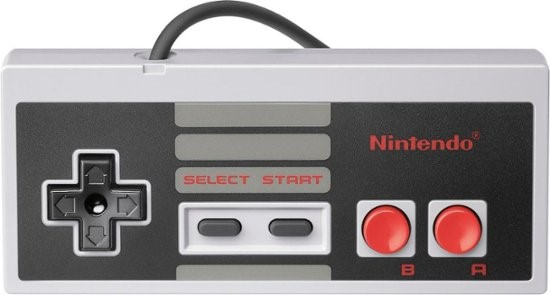
\includegraphics[width=0.62\textwidth]{nes_controller.jpg}
  \caption{NES controller}
  \label{fig:nes_controller}
\end{figure}

\begin{figure}
  \centering
  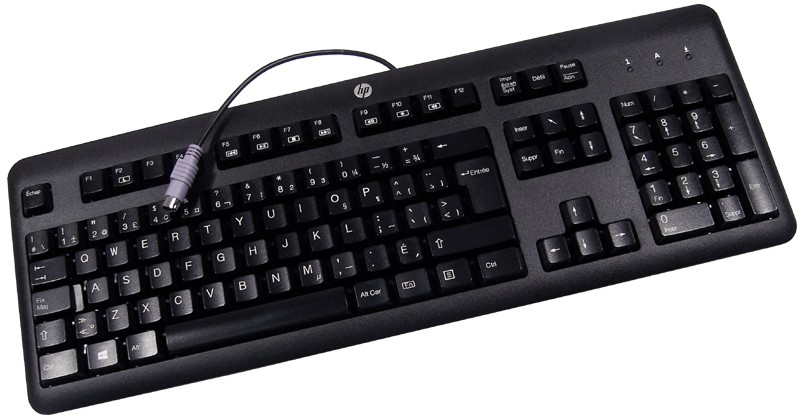
\includegraphics[width=0.75\textwidth]{ps2_keyboard.jpg}
  \caption{PS/2 keyboard}
  \label{fig:ps2_keyboard}
\end{figure}

\begin{figure}
  \centering
  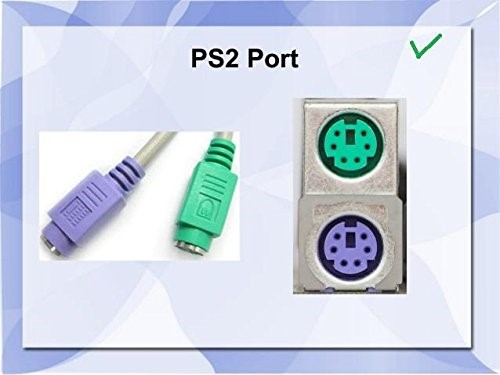
\includegraphics[width=0.75\textwidth]{ps2_port.jpg}
  \caption{PS/2 port}
  \label{fig:ps2_port}
\end{figure}

\begin{figure}
  \centering
  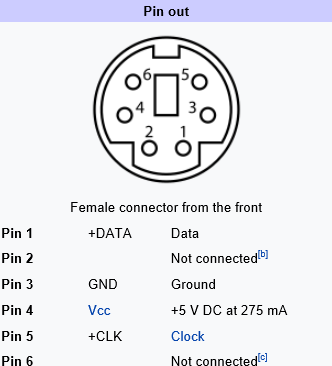
\includegraphics[width=0.5\textwidth]{ps2_port_6_pin_mini_din_connector.png}
  \caption{PS/2 port 6-pin mini-DIN connector}
  \label{fig:ps2_port_6_pin_mini_din_connector}
\end{figure}

\begin{figure}
  \centering
  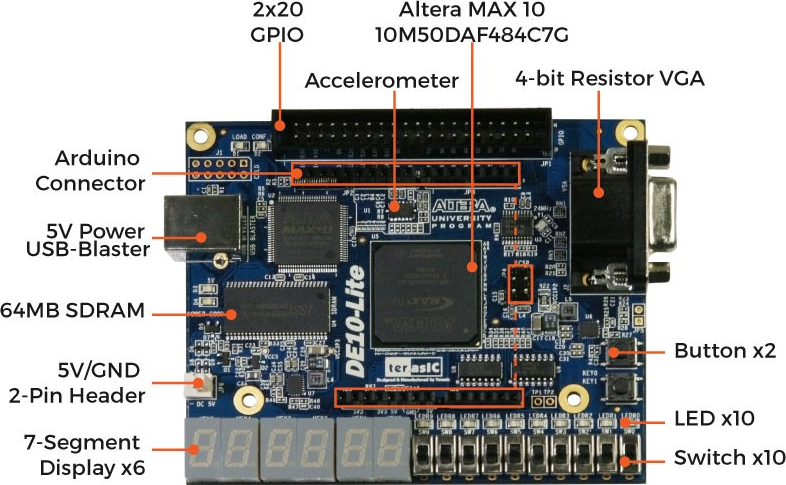
\includegraphics[width=0.85\textwidth]{de10_lite.jpg}
  \caption{ECE 272 DE10-Lite FPGA courtesy of the EECS department at OSU}
  \label{fig:de10_lite}
\end{figure}

\begin{figure}
  \centering
  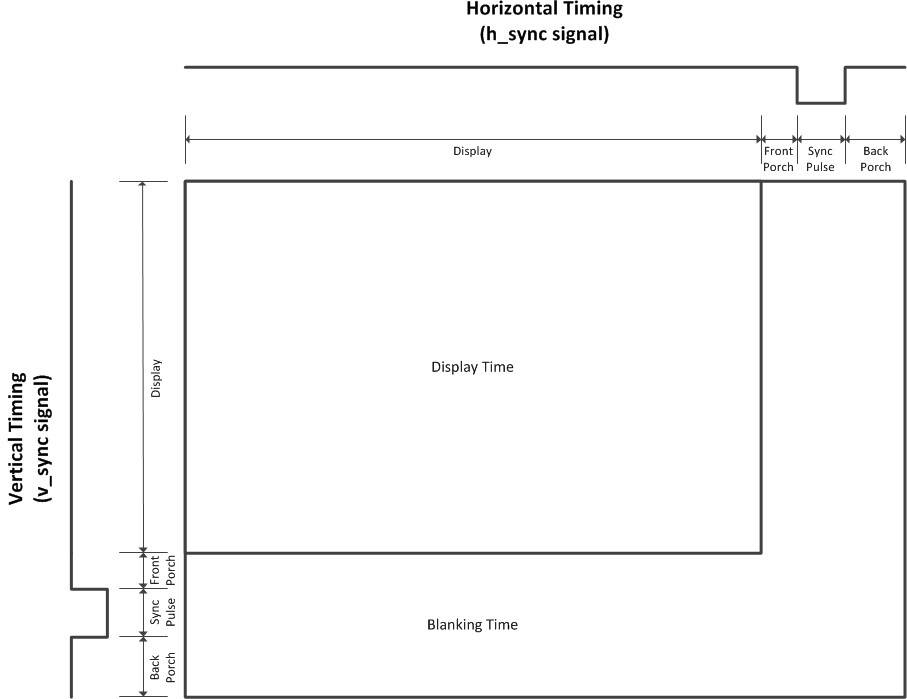
\includegraphics[width=0.75\textwidth]{vga_timing_sequence.png}
  \caption{Timing specifications and pixel range of the VGA output}
  \label{fig:vga_timing_sequence}
\end{figure}

%%%%%%%%%%%%%%%%%%%%%%%%%%%%%%%%%%%%%%%%%%%%%%%%%%%%%%%%%%%%%%%%%%%%%%%%%%%%%%%%
% High-Level Description
%%%%%%%%%%%%%%%%%%%%%%%%%%%%%%%%%%%%%%%%%%%%%%%%%%%%%%%%%%%%%%%%%%%%%%%%%%%%%%%%
\section{High-Level Description}

%%%%%%%%%%%%%%%%%%%%%%%%%%%%%%%%%%%%%%%%
% Top-Level Hardware Diagram
%%%%%%%%%%%%%%%%%%%%%%%%%%%%%%%%%%%%%%%%
\subsection{Top-Level Hardware Diagram}

\begin{figure}[ht]
  \centering
  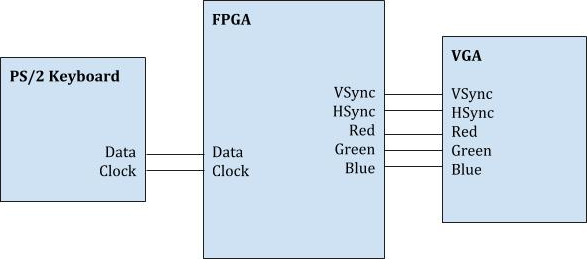
\includegraphics[width=0.75\textwidth]{ps2_top_level_block_diagram.jpg}
  \caption{Top-level hardware diagram for PS/2 keyboard}
  \label{fig:ps2_top_level_block_diagram}
\end{figure}

Inputs: The FPGA reads in data and clock signals from the PS/2 keyboard.

Outputs: The FPGA outputs VSync, HSync signals as well as Red, Green, and Blue values to display as a VGA image.

Description: The top-level hardware diagram above shows that the DE10-Lite takes in a Data and Clock signal from the PS/2 Keyboard. Then, it manipulates that data to form five outputs required for a VGA image.

\begin{figure}[ht]
  \centering
  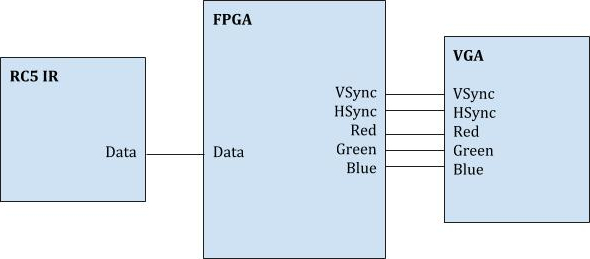
\includegraphics[width=0.75\textwidth]{ir_top_level_block_diagram.jpg}
  \caption{Top-level hardware diagram for RC5 IR}
  \label{fig:ir_top_level_block_diagram}
\end{figure}

Inputs: The FPGA reads in a data signal from RC5 IR.

Outputs: The FPGA outputs VSync, HSync signals as well as Red, Green, and Blue values to display as a VGA image.

Description: The top-level hardware diagram above shows that the DE10-Lite takes in a Data signal in the form of RC5 IR. Then, the FPGA manipulates that data to form five outputs required for a VGA image.

\begin{figure}[ht]
  \centering
  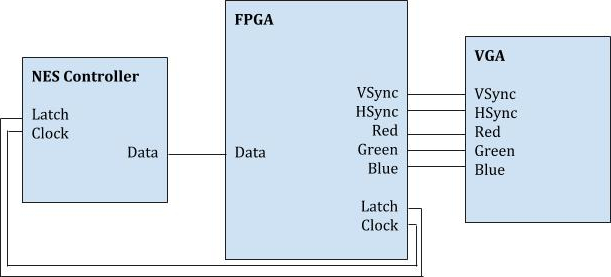
\includegraphics[width=0.75\textwidth]{nes_top_level_block_diagram.jpg}
  \caption{Top-level hardware diagram for NES controller}
  \label{fig:nes_top_level_block_diagram}
\end{figure}

Inputs: The FPGA reads Latch, Clock, and Data signals from the NES Controller.

Outputs: The FPGA outputs VSync, HSync signals as well as Red, Green, and Blue values to display as a VGA image.

Description: The top-level hardware diagram above shows that the DE10-Lite takes in a Data, Latch, and Clock signal from the NES Controller. Then, the FPGA manipulates that data to form five outputs required for a VGA image.

%%%%%%%%%%%%%%%%%%%%%%%%%%%%%%%%%%%%%%%%
% Top-Level HDL Diagram
%%%%%%%%%%%%%%%%%%%%%%%%%%%%%%%%%%%%%%%%
\subsection{Top-Level Hardware Diagram}

\begin{figure}[ht]
  \centering
  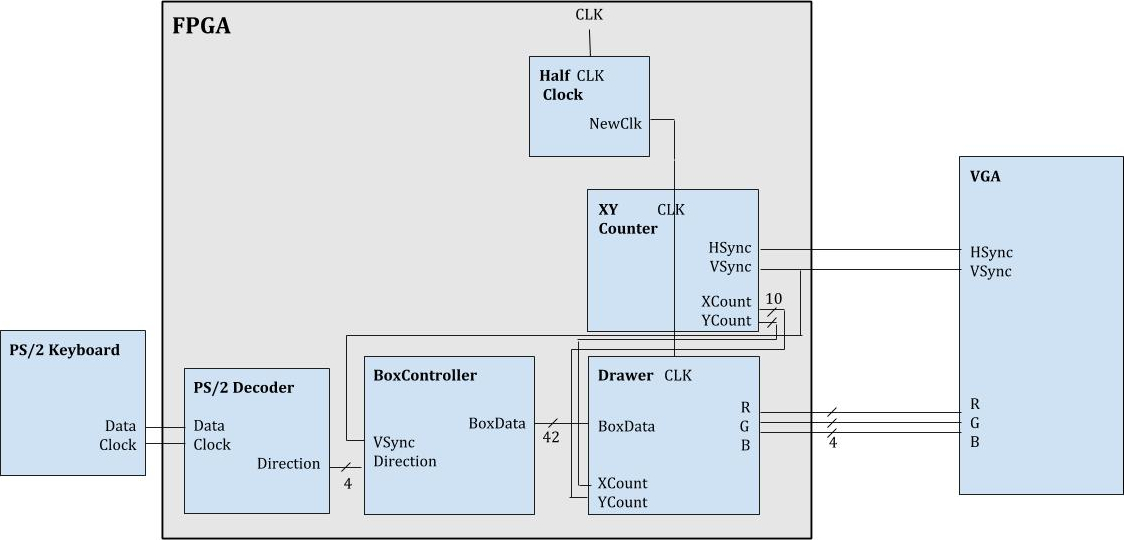
\includegraphics[width=\textwidth]{hdl_top_level.jpg}
  \caption{Top-level HDL diagram for PS/2 keyboard}
  \label{fig:hdl_top_level}
\end{figure}

\begin{figure}[ht]
  \centering
  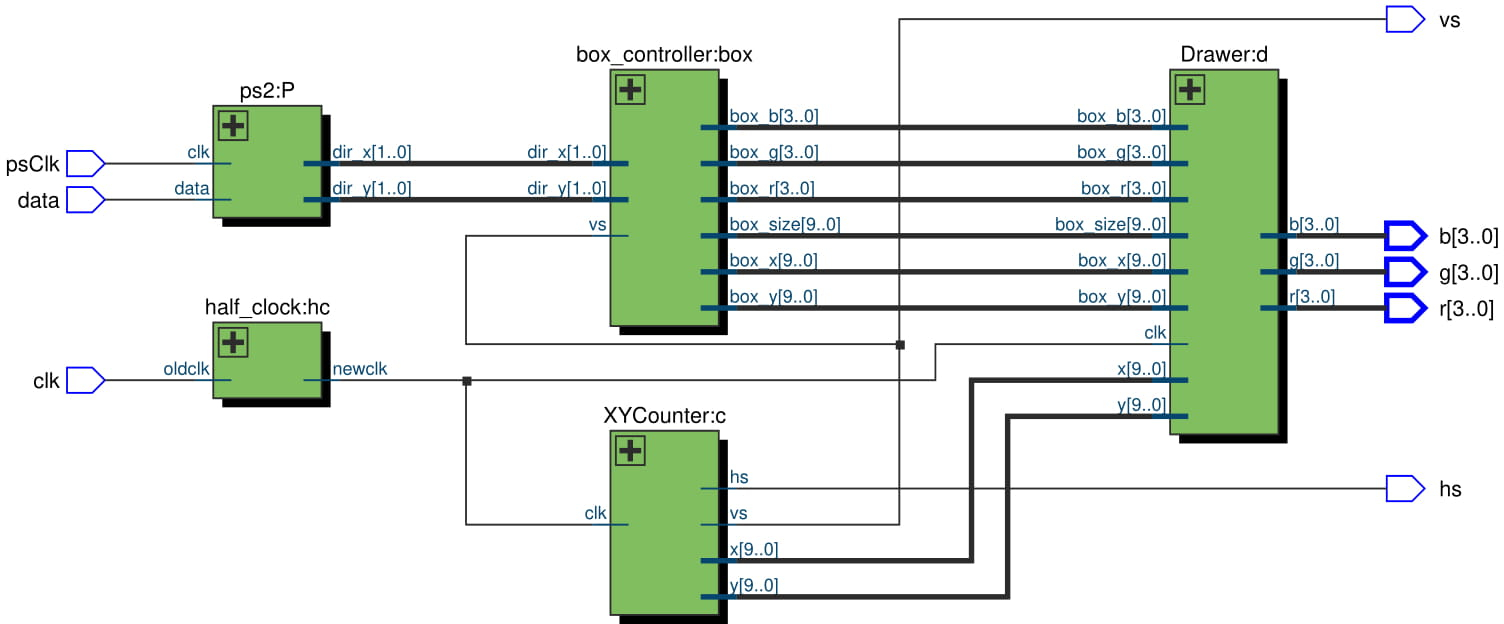
\includegraphics[width=\textwidth]{ps2_top_level.jpg}
  \caption{Top-level diagram for PS/2 keyboard}
  \label{fig:ps2_top_level}
\end{figure}

\begin{figure}
  \centering
  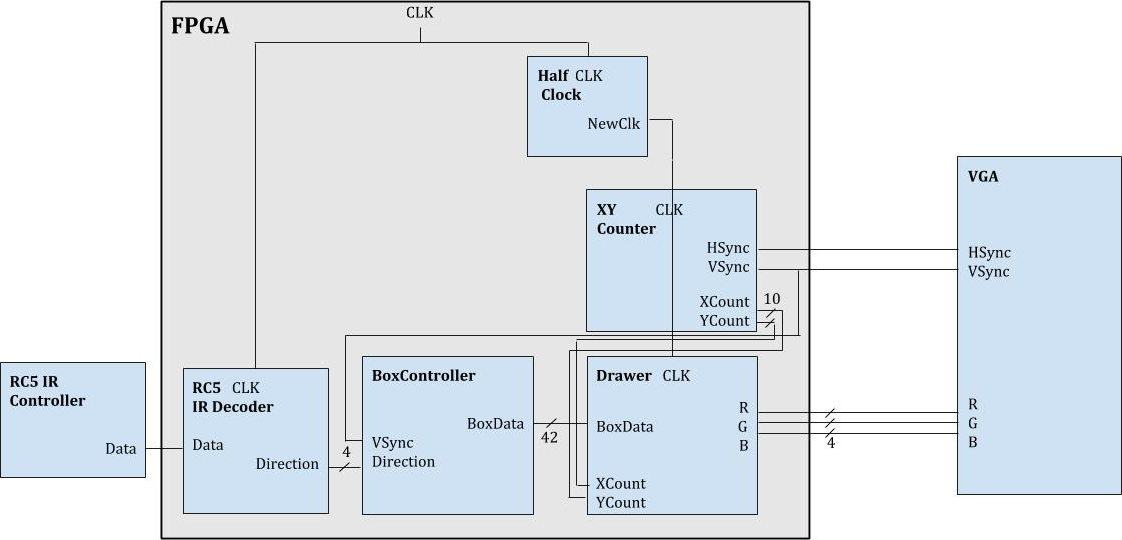
\includegraphics[width=\textwidth]{ir_hdl_top_level.jpg}
  \caption{Top-level HDL diagram for RC5 IR}
  \label{fig:ir_hdl_top_level}
\end{figure}

\begin{figure}
  \centering
  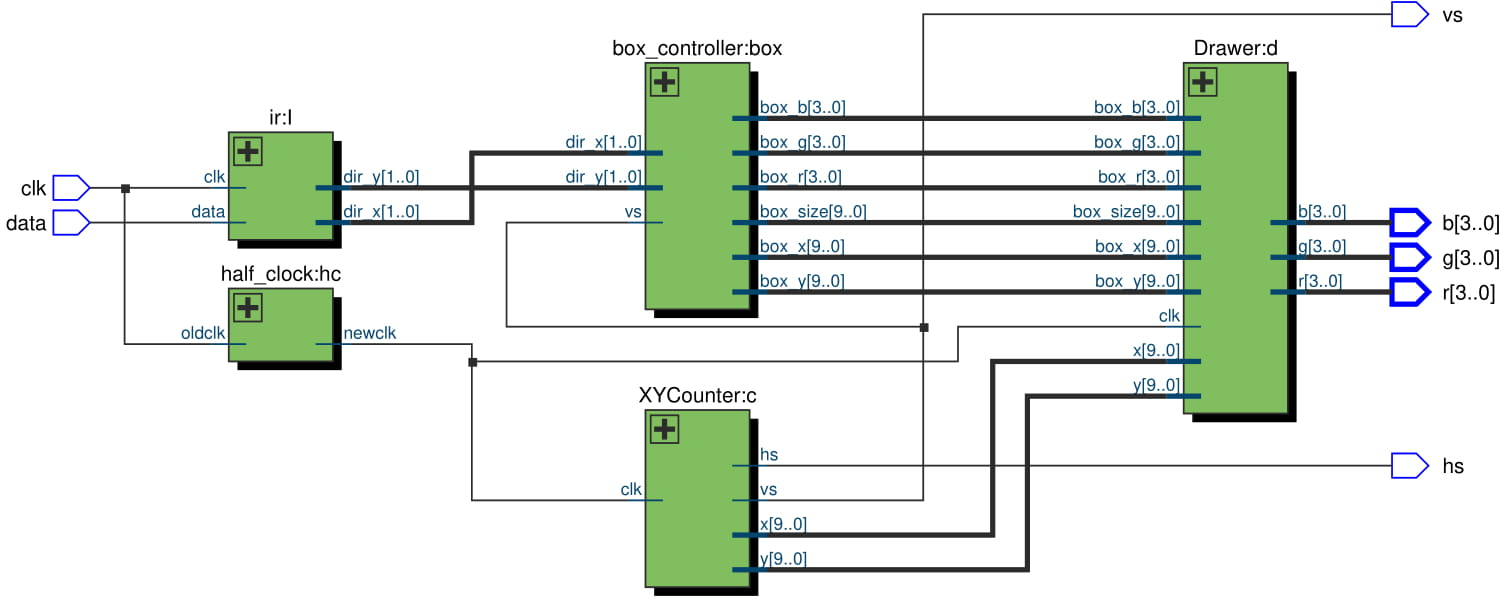
\includegraphics[width=\textwidth]{ir_top_level.jpg}
  \caption{Top-level diagram for RC5 IR}
  \label{fig:ir_top_level}
\end{figure}

\begin{figure}
  \centering
  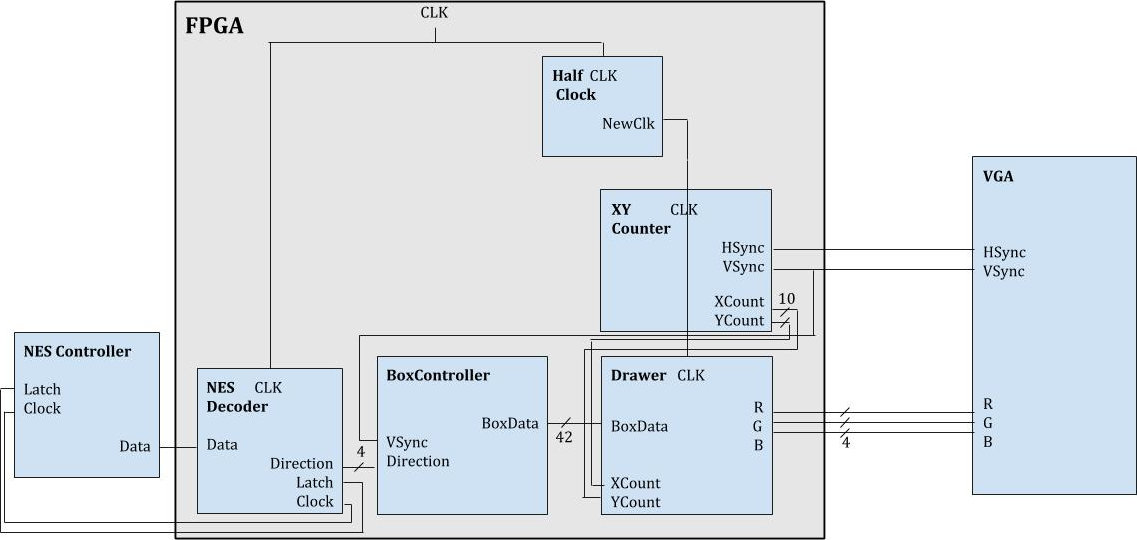
\includegraphics[width=\textwidth]{nes_hdl_top_level.jpg}
  \caption{Top-level HDL diagram for NES controller}
  \label{fig:nes_hdl_top_level}
\end{figure}

\begin{figure}
  \centering
  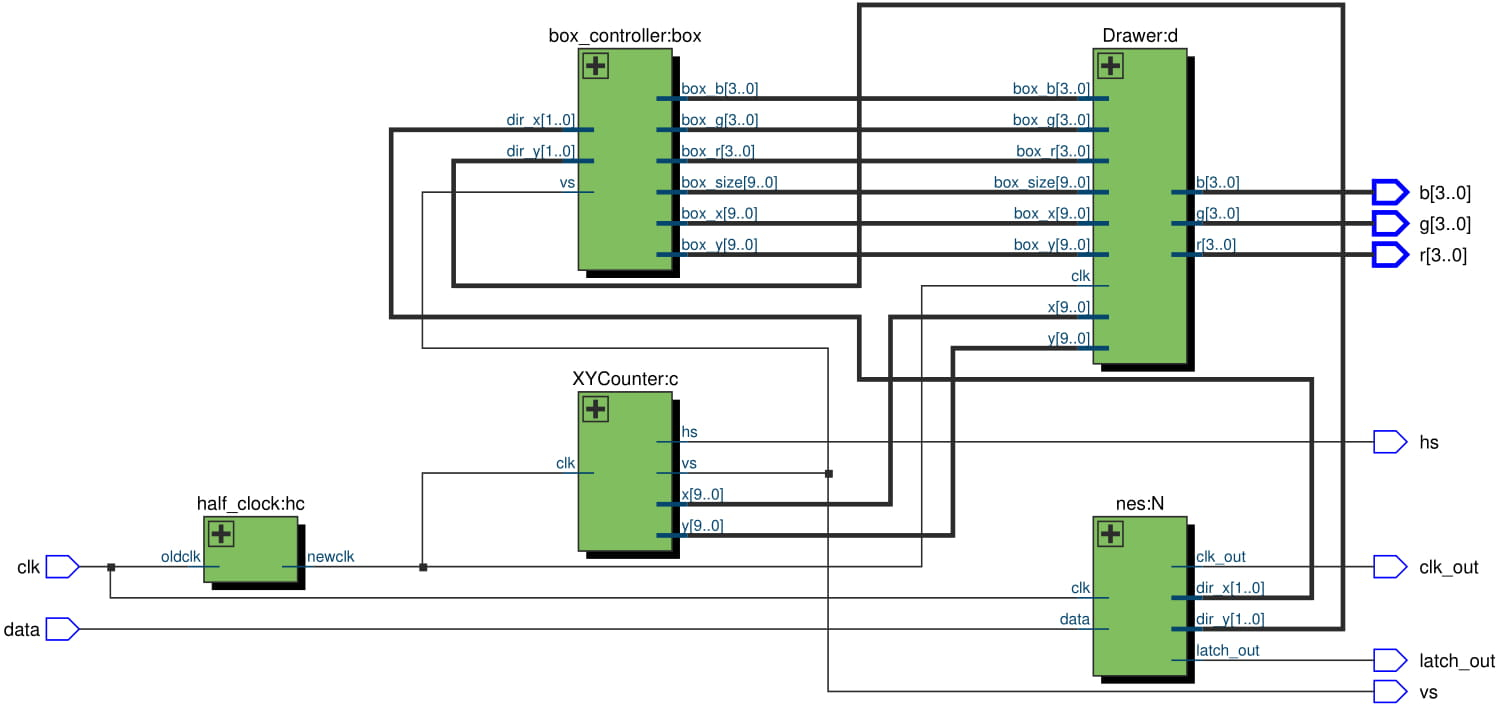
\includegraphics[width=\textwidth]{nes_top_level.jpg}
  \caption{Top-level diagram for NES controller}
  \label{fig:nes_top_level}
\end{figure}

%%%%%%%%%%%%%%%%%%%%%%%%%%%%%%%%%%%%%%%%%%%%%%%%%%%%%%%%%%%%%%%%%%%%%%%%%%%%%%%%
% Controllers
%%%%%%%%%%%%%%%%%%%%%%%%%%%%%%%%%%%%%%%%%%%%%%%%%%%%%%%%%%%%%%%%%%%%%%%%%%%%%%%%
\section{Controllers}

%%%%%%%%%%%%%%%%%%%%%%%%%%%%%%%%%%%%%%%%
% PS/2 Keyboard
%%%%%%%%%%%%%%%%%%%%%%%%%%%%%%%%%%%%%%%%
\subsection{PS/2}

The PS/2 port is a 6-pin mini-DIN connector used for connecting keyboards or mice to a computer system. It was first designed by IBM in 1987. A mini-DIN connector refers to a family of multi-pin electrical connectors used in a variety of environments. They are 9.5 millimeters in diameter and come in seven patterns ranging from three to nine pins. PS/2 ports have serial, synchronous, and bidirectional communication in which the attached device generates a clock signal while the host controls communication along the clock line. When the clock is LOW, communication from the PS/2 port is prevented. The assignments of each pin on the 6-pin connector are illustrated clearly in Figure~\ref{fig:ps2_port_6_pin_mini_din_connector}, which can be found on page~\pageref{fig:ps2_port_6_pin_mini_din_connector}.

%%%%%%%%%%%%%%%%%%%%%%%%%%%%%%%%%%%%%%%%
% RC5 IR
%%%%%%%%%%%%%%%%%%%%%%%%%%%%%%%%%%%%%%%%
\subsection{RC5 IR}

RC5 IR refers to a protocol developed by Phillips in the late 1980’s as a consumer infrared remote control communication code for consumer electronics. The RC5 uses a bi-phase coding with a frequency of 36 kHz and is comprised of a keypad and a transmitter integrated circuit, which drives an infrared LED. The transmission of data starts with two bits followed by a toggle bit, which changes value upon a each key-press. There are five address bits, which indicate the device that is being controlled. Lastly, the six commands bits represent the data that is to be transmitted from the RC5 to the device.

%%%%%%%%%%%%%%%%%%%%%%%%%%%%%%%%%%%%%%%%
% NES Controller
%%%%%%%%%%%%%%%%%%%%%%%%%%%%%%%%%%%%%%%%
\subsection{NES Controller}

The NES Controller is an 8-bit controller developed by Nintendo in the 1980’s. The device transmits 8-bits of data, which equates to one bit for each of the buttons on the controller: A, B, Select, Start, Up, Down, Left, and Right. The NES controller also contains a latch to store the state of buttons internally as well as a clock. Every 60 Hz, the NES sends a 12 microsecond signal to the latch, indicating that it must store the state of all eight buttons. Following the Latch signal, 8 clock pulses are emitted, one for each button on the controller. If the button is pressed upon the rising edge of the pulse, data is asserted to ground. This means that in the NES controller, the buttons are active low because Data asserts to ground when the button is pressed.

%%%%%%%%%%%%%%%%%%%%%%%%%%%%%%%%%%%%%%%%%%%%%%%%%%%%%%%%%%%%%%%%%%%%%%%%%%%%%%%%
% HDL Modules
%%%%%%%%%%%%%%%%%%%%%%%%%%%%%%%%%%%%%%%%%%%%%%%%%%%%%%%%%%%%%%%%%%%%%%%%%%%%%%%%
\section{HDL Modules}

%%%%%%%%%%%%%%%%%%%%%%%%%%%%%%%%%%%%%%%%
% PS/2 Modules
%%%%%%%%%%%%%%%%%%%%%%%%%%%%%%%%%%%%%%%%
\subsection{PS/2 Modules}

%%%%%%%%%%%%%%%%%%%%
% PS/2 Decoder
%%%%%%%%%%%%%%%%%%%%
\subsubsection{PS/2 Decoder}

\begin{figure}[ht]
  \centering
  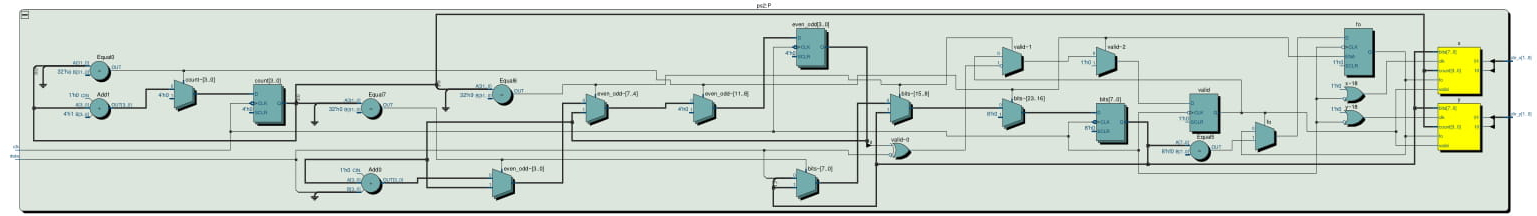
\includegraphics[width=\textwidth]{ps2.jpg}
  \caption{PS/2 keyboard decoder}
  \label{fig:ps2}
\end{figure}

\begin{figure}[ht]
  \centering
  \includegraphics[width=\textwidth]{ps2_simulation_1st_conditional.png}
  \caption{PS/2 module’s simulation testing - Keypress W (up)}
  \label{fig:ps2_simulation_1st_conditional}
\end{figure}

\newpage

\begin{figure}[ht]
  \centering
  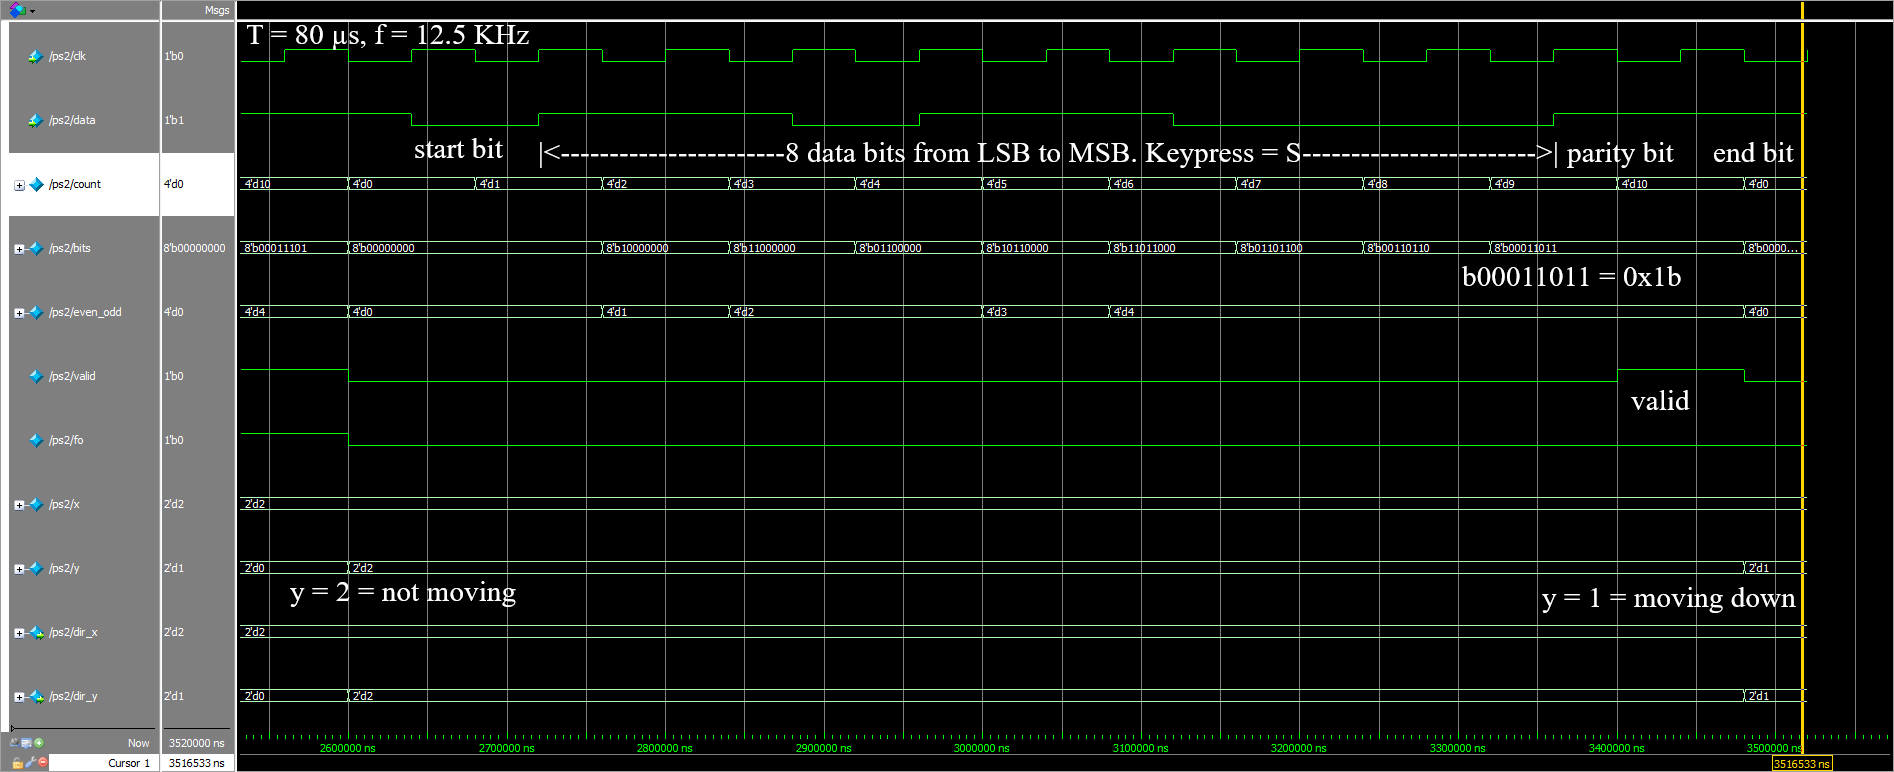
\includegraphics[width=\textwidth]{ps2_simulation_3rd_conditional.png}
  \caption{PS/2 module’s simulation testing - Keypress S (down)}
  \label{fig:ps2_simulation_3rd_conditional}
\end{figure}

\begin{figure}[ht]
  \centering
  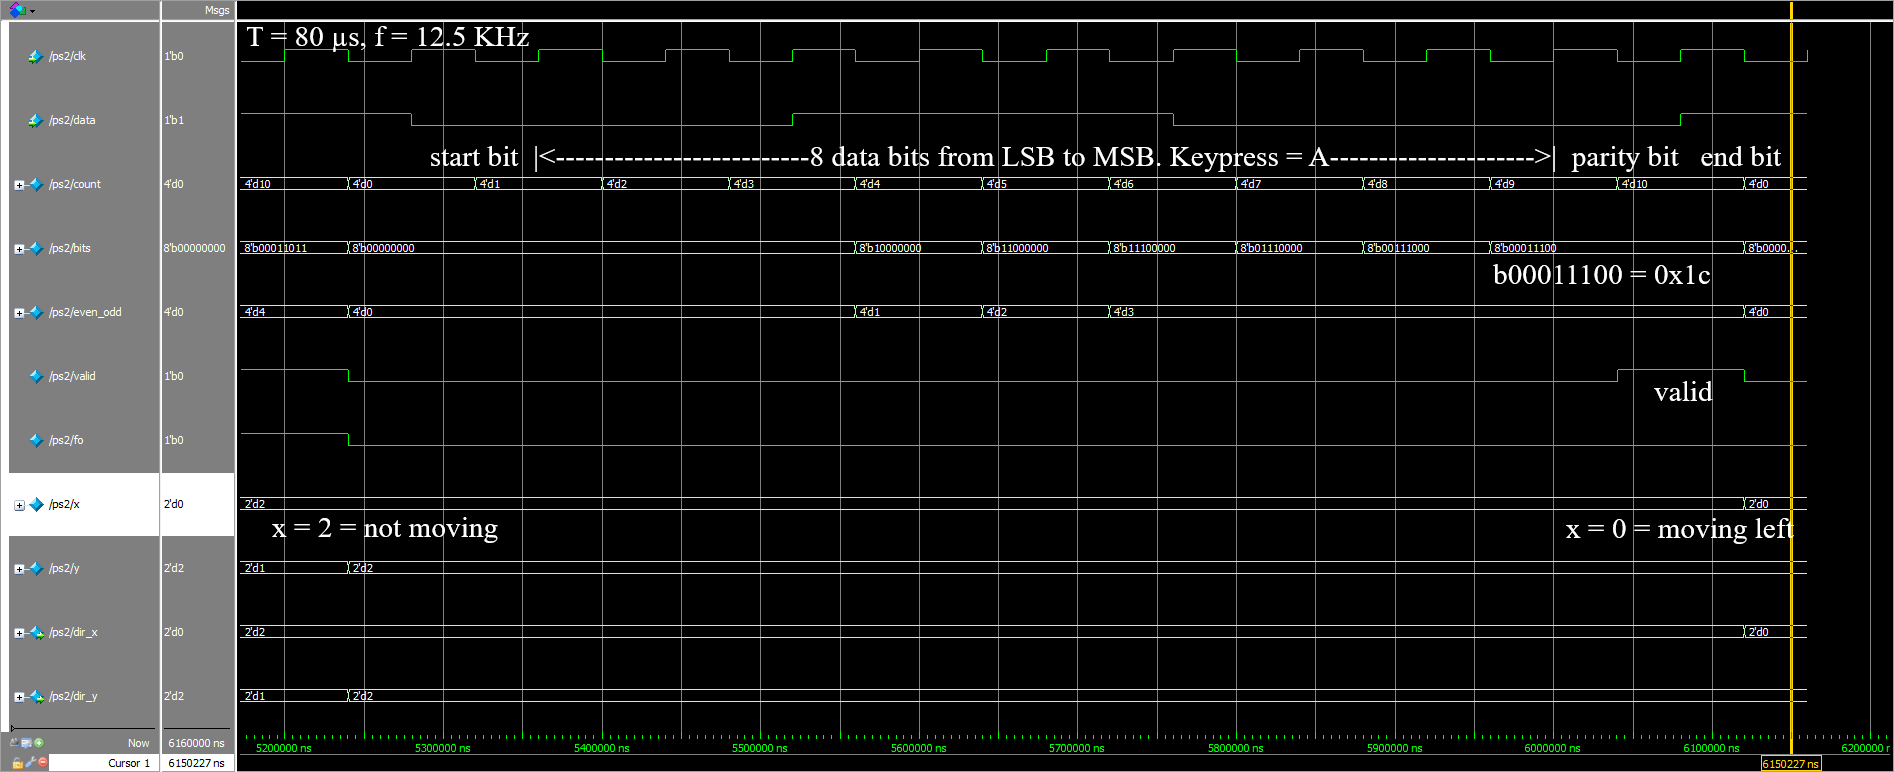
\includegraphics[width=\textwidth]{ps2_simulation_5th_conditional.png}
  \caption{PS/2 module’s simulation testing - Keypress A (left)}
  \label{fig:ps2_simulation_5th_conditional}
\end{figure}

\newpage

\begin{figure}[ht]
  \centering
  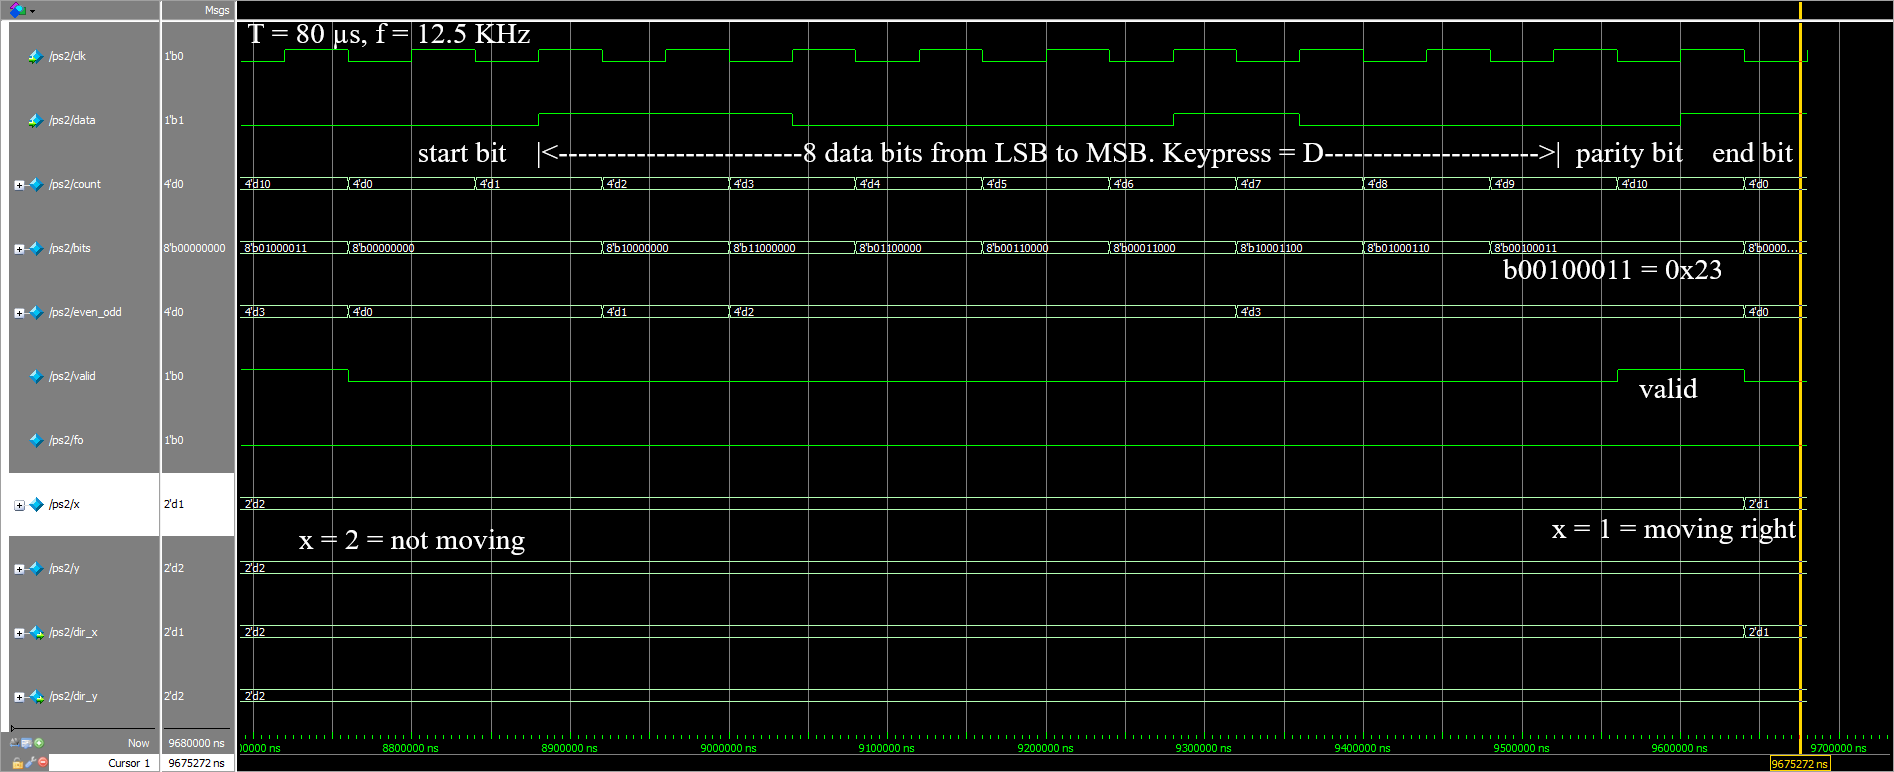
\includegraphics[width=\textwidth]{ps2_simulation_7th_conditional.png}
  \caption{PS/2 module’s simulation testing - Keypress D (right)}
  \label{fig:ps2_simulation_7th_conditional}
\end{figure}

\begin{figure}[ht]
  \centering
  \includegraphics[width=\textwidth]{ps2_simulation_9th_conditional_key_released.png}
  \caption{PS/2 module’s simulation testing - Key release signal (0xF0)}
  \label{fig:ps2_simulation_9th_conditional_key_released}
\end{figure}

Inputs: Clock and Data signal.

Outputs: Two buses to represent the box’s movement in the $x$ and $y$ direction.

Description: The PS/2 keyboard decoder module begins with an always flip flop on the negative edge of the clock signal, indicating that the data values are generated only after the clock has gone to low. The module then determines the value of \mintinline{text}{count}, which continuously increments between 0 and 10. If the value of \mintinline{text}{count} is 10, then the keyboard inputs, recognized as A, W, S, and D, and translated into variables representing the movement and direction of the box image. If the \mintinline{text}{count} is between 1 and 8, then data from the PS/2 keyboard is simply stored until \mintinline{text}{count} returns to 10, in which the values are then outputted to directional values stored in the variables \mintinline{text}{dir_x} and \mintinline{text}{dir_y}.

%%%%%%%%%%%%%%%%%%%%%%%%%%%%%%%%%%%%%%%%
% RC5 IR Modules
%%%%%%%%%%%%%%%%%%%%%%%%%%%%%%%%%%%%%%%%
\subsection{RC5 IR Modules}

%%%%%%%%%%%%%%%%%%%%
% RC5 IR Decoder
%%%%%%%%%%%%%%%%%%%%
\subsubsection{RC5 IR Decoder}

\begin{figure}[ht]
  \centering
  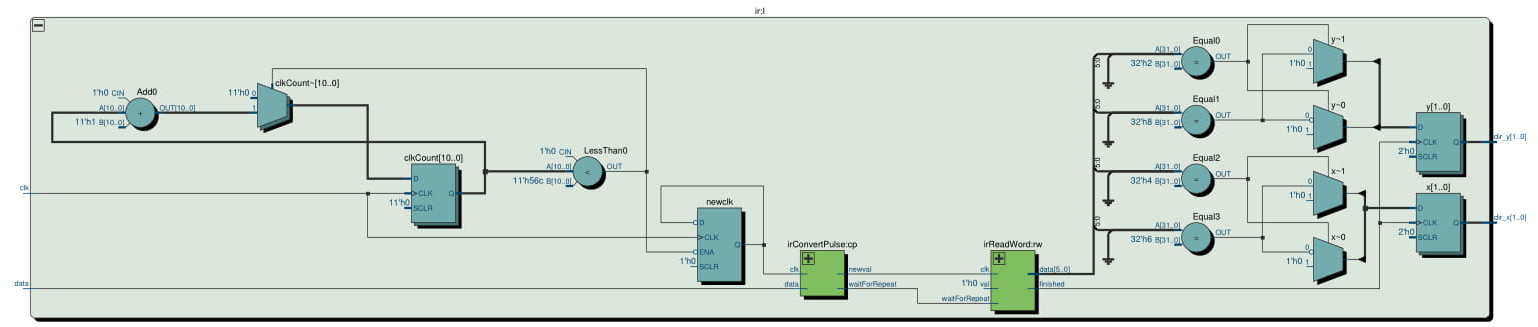
\includegraphics[width=\textwidth]{ir.jpg}
  \caption{RC5 IR decoder}
  \label{fig:ir}
\end{figure}

\begin{figure}[ht]
  \centering
  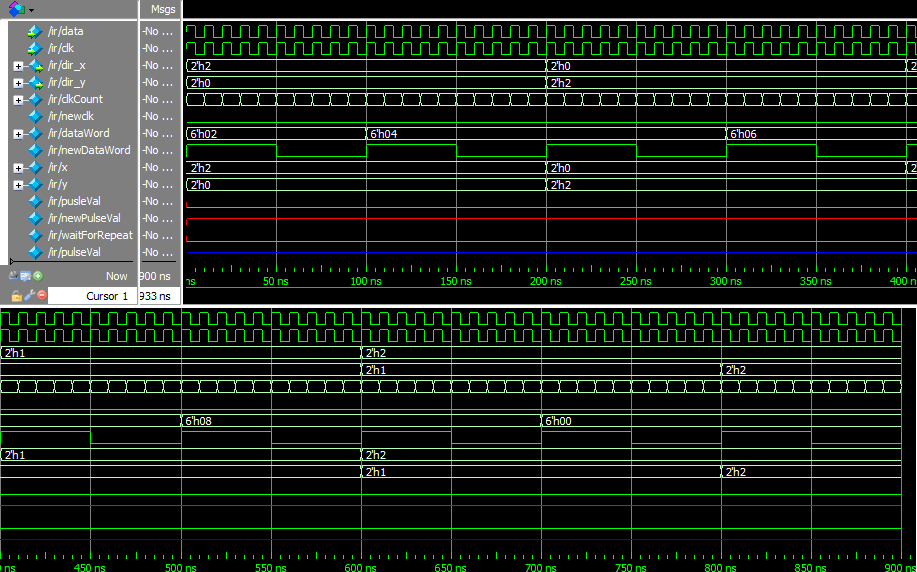
\includegraphics[width=\textwidth]{ir_decoder_simulation.png}
  \caption{RC5 IR decoder decoding up, down, left, right, and neutral direction controls from data word}
  \label{fig:ir_decoder_simulation}
\end{figure}

Inputs: Clock and Data signal.

Outputs: Two buses to represent the box’s movement in the $x$ and $y$ direction.

Description: The first step in designing the RC5 IR module was slowing the normal FPGA clock frequency of 50 MHz to 36 KHz, the frequency used in RC5 data transmission. RC5 works by using bi-phase encoding, meaning that during each clock period, there is either a 1 or 0, where 1 represents a rising edge and 0 represents a falling edge. Next, the ConvertPulse and ReadData modules were instantiated. Convert Pulse takes in the 32-bit pulse emitted by the RC5 and treats the entire pulse as HIGH and the absence of a pulse as LOW. Then, when the pulse signal encoding and bi-phase encoding are decoded, a 14-bit result follows. The first 2-bits are start bits and represent when a new data transmission occurs. The toggle is unaffected if no new button is pressed. However, if a new data line is activated, the toggle bit changes. The next 5-bits are address bits to indicate the path to a device that is being transmitted to. Lastly, 6-bits are used to represent the transmitted data. In our module, the encodings used to represent the direction and

%%%%%%%%%%%%%%%%%%%%
% RC5 IR Convert Pulse
%%%%%%%%%%%%%%%%%%%%
\subsubsection{RC5 IR Convert Pulse}

\begin{figure}[ht]
  \centering
  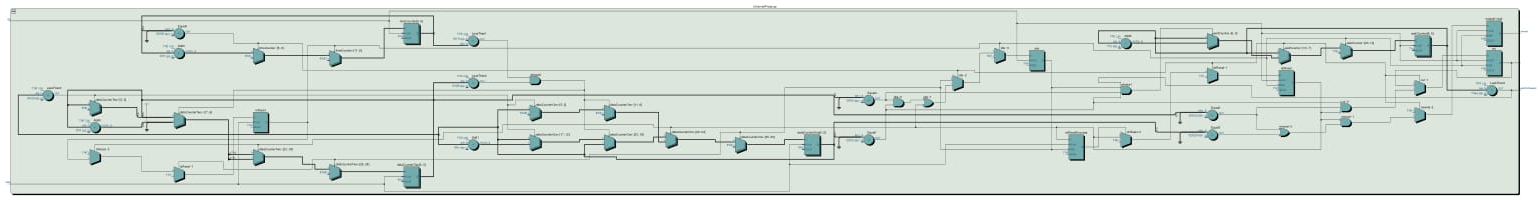
\includegraphics[width=\textwidth]{irconvertpulse.jpg}
  \caption{IR convert pulse}
  \label{fig:irconvertpulse}
\end{figure}

\begin{figure}[ht]
  \centering
  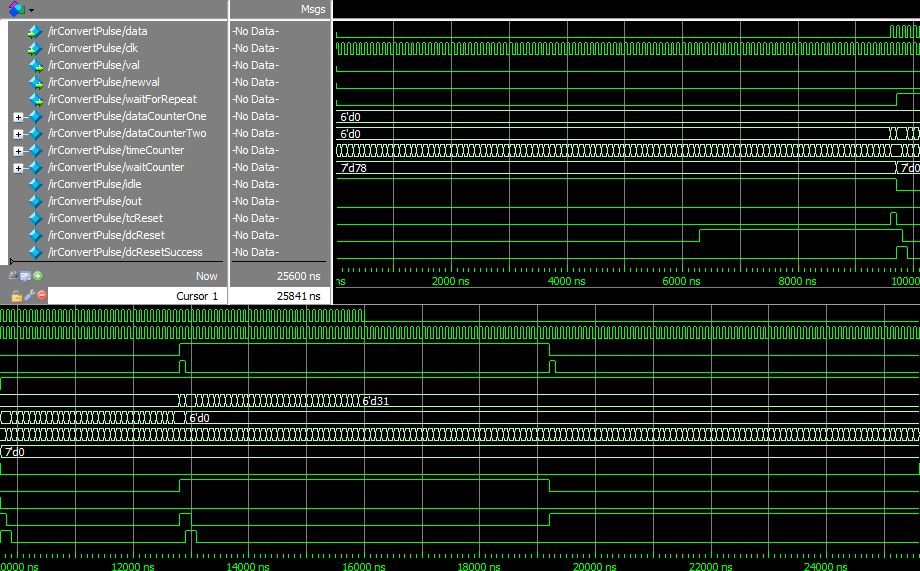
\includegraphics[width=\textwidth]{ir_simulation_convertpulse.png}
  \caption{Testing conversion of inputs from idle to HIGH to LOW}
  \label{fig:ir_simulation_convertpulse}
\end{figure}

Description: The module above converts the encoded pulse outputted in bi-phase encoding by RC5 IR into binary form.

%%%%%%%%%%%%%%%%%%%%
% RC5 IR Read Word
%%%%%%%%%%%%%%%%%%%%
\subsubsection{RC5 IR Read Word}

\begin{figure}[ht]
  \centering
  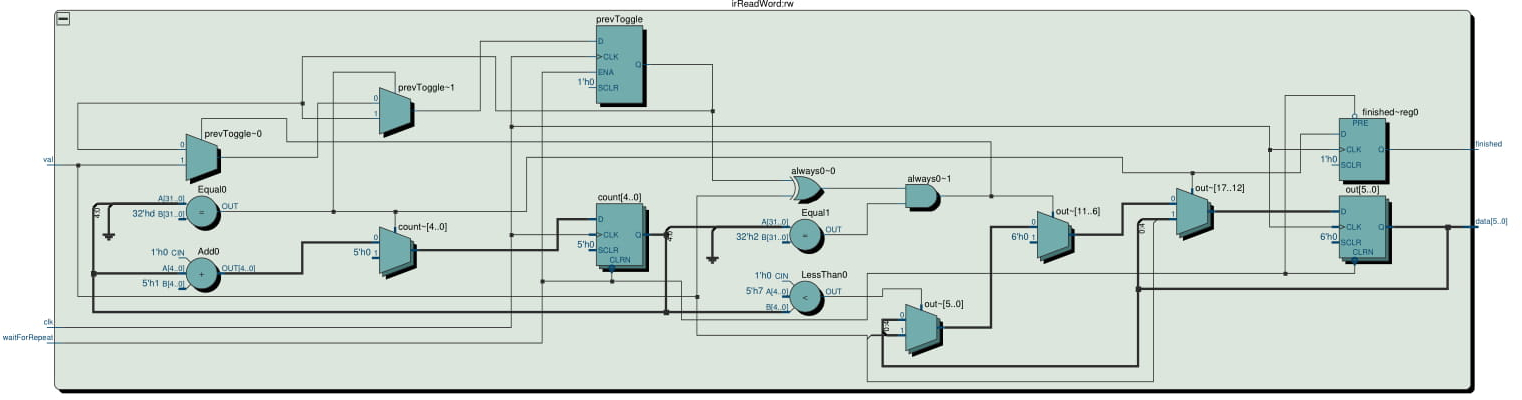
\includegraphics[width=\textwidth]{irreadword.jpg}
  \caption{IR read word}
  \label{fig:irreadword}
\end{figure}

\begin{figure}[ht]
  \centering
  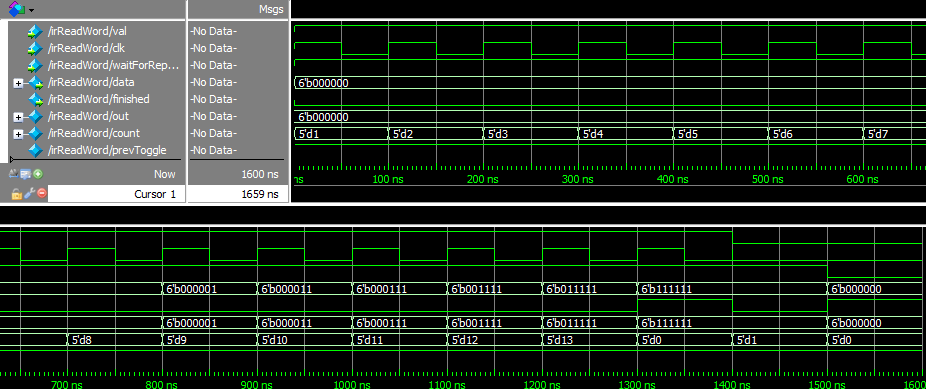
\includegraphics[width=\textwidth]{ir_simulation_readword.png}
  \caption{Readind data word ``111111'' then resetting}
  \label{fig:ir_simulation_readword}
\end{figure}

Description: The module above converts encoded binary into data.

\newpage

%%%%%%%%%%%%%%%%%%%%%%%%%%%%%%%%%%%%%%%%
% NES Modules
%%%%%%%%%%%%%%%%%%%%%%%%%%%%%%%%%%%%%%%%
\subsection{NES Modules}

%%%%%%%%%%%%%%%%%%%%
% NES Decoder
%%%%%%%%%%%%%%%%%%%%
\subsubsection{NES Decoder}

\begin{figure}[ht]
  \centering
  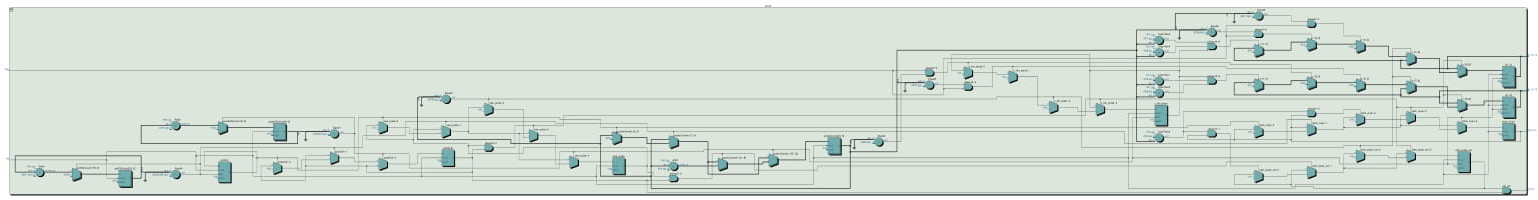
\includegraphics[width=\textwidth]{nes.jpg}
  \caption{NES controller decoder}
  \label{fig:nes}
\end{figure}

\begin{figure}[ht]
  \centering
  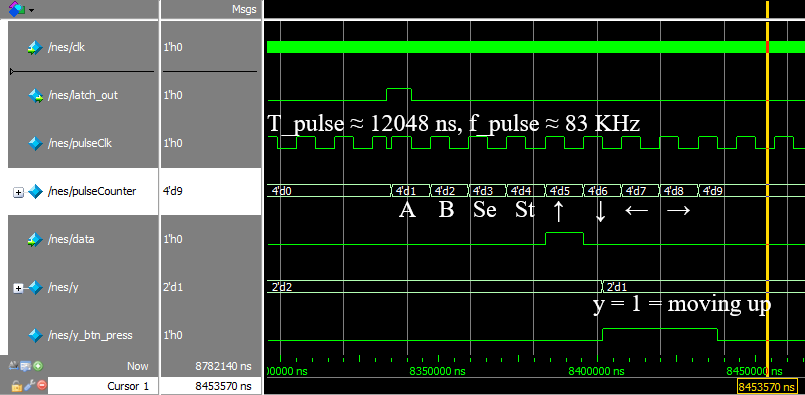
\includegraphics[width=\textwidth]{nes_simulation_moving_up.png}
  \caption{NES module’s simulation testing - Moving up keypress}
  \label{fig:nes_simulation_moving_up}
\end{figure}

Inputs: Clock and Data signal.

Outputs: Two buses to represent the box’s movement in the $x$ and $y$ direction. Also outputs new clock signal and latch data.

Description: Initially, the decoder sends a latch output to the controller. Every 60Hz, the decoder asserts the latch for 12 microseconds, which stabilizes each buttons state. For this module, a clock slowing mechanism was inserted so that the internal clock of the FPGA, which is naturally 50MHz, can be used. On the falling edge of the latch, the decoder reads the first value, which is A. Six microseconds after, it begins sending 8 clock pulses which have a period of 12 microseconds. On every rising edge of the clock, the decoder cycles to the next button value, for a total of eight button values. The value is then read on the falling edge of that cycle and stored in module variables. Since the only button actions which affect our box image are the up, down, left, and right arrows, those are the only ones that are stored and sent to different modules.

%%%%%%%%%%%%%%%%%%%%%%%%%%%%%%%%%%%%%%%%
% General Modules Used in Each Design
%%%%%%%%%%%%%%%%%%%%%%%%%%%%%%%%%%%%%%%%
\subsection{General Modules Used in Each Design}

%%%%%%%%%%%%%%%%%%%%
% Clock Frequency Module
%%%%%%%%%%%%%%%%%%%%
\subsubsection{Clock Frequency Module}

\begin{figure}[ht]
  \centering
  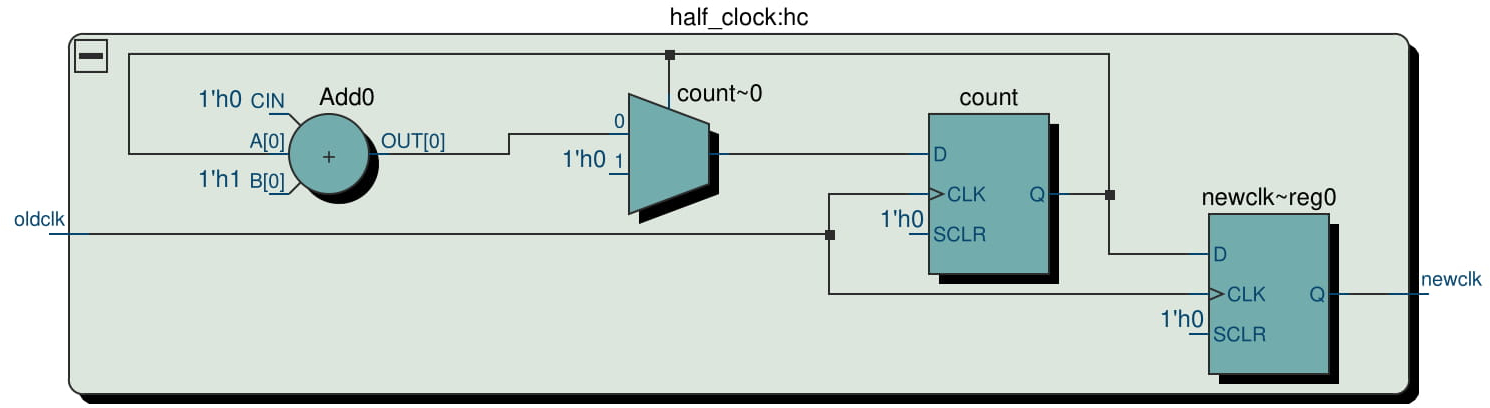
\includegraphics[width=\textwidth]{half_clock.jpg}
  \caption{Half clock module}
  \label{fig:half_clock}
\end{figure}

\begin{figure}[ht]
  \centering
  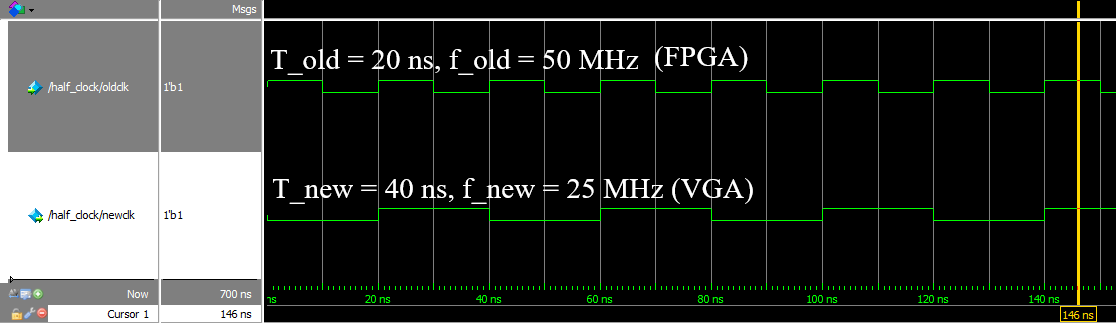
\includegraphics[width=\textwidth]{half_clock_simulation.png}
  \caption{Half clock module’s simulation testing - Making a half-as-fast clock}
  \label{fig:half_clock_simulation}
\end{figure}

Inputs: \mintinline{text}{oldClock} signal.

Outputs: \mintinline{text}{newClock} signal representing a clock with half the frequency of \mintinline{text}{oldClock}.

Description: The clock module plays an essential role in allowing the output to be displayed as VGA. The natural frequency of the DE10-Lite is 50 MHz. However, the pixel clode on the VGA mode timing specifications is 25 MHz. Because of this difference, a half clock module is required to half the clock frequency of the FPGA so that it corresponds with the pixel clock at 25 MHz.

\newpage

%%%%%%%%%%%%%%%%%%%%
% Box Controller Module
%%%%%%%%%%%%%%%%%%%%
\subsubsection{Box Controller Module}

\begin{figure}[ht]
  \centering
  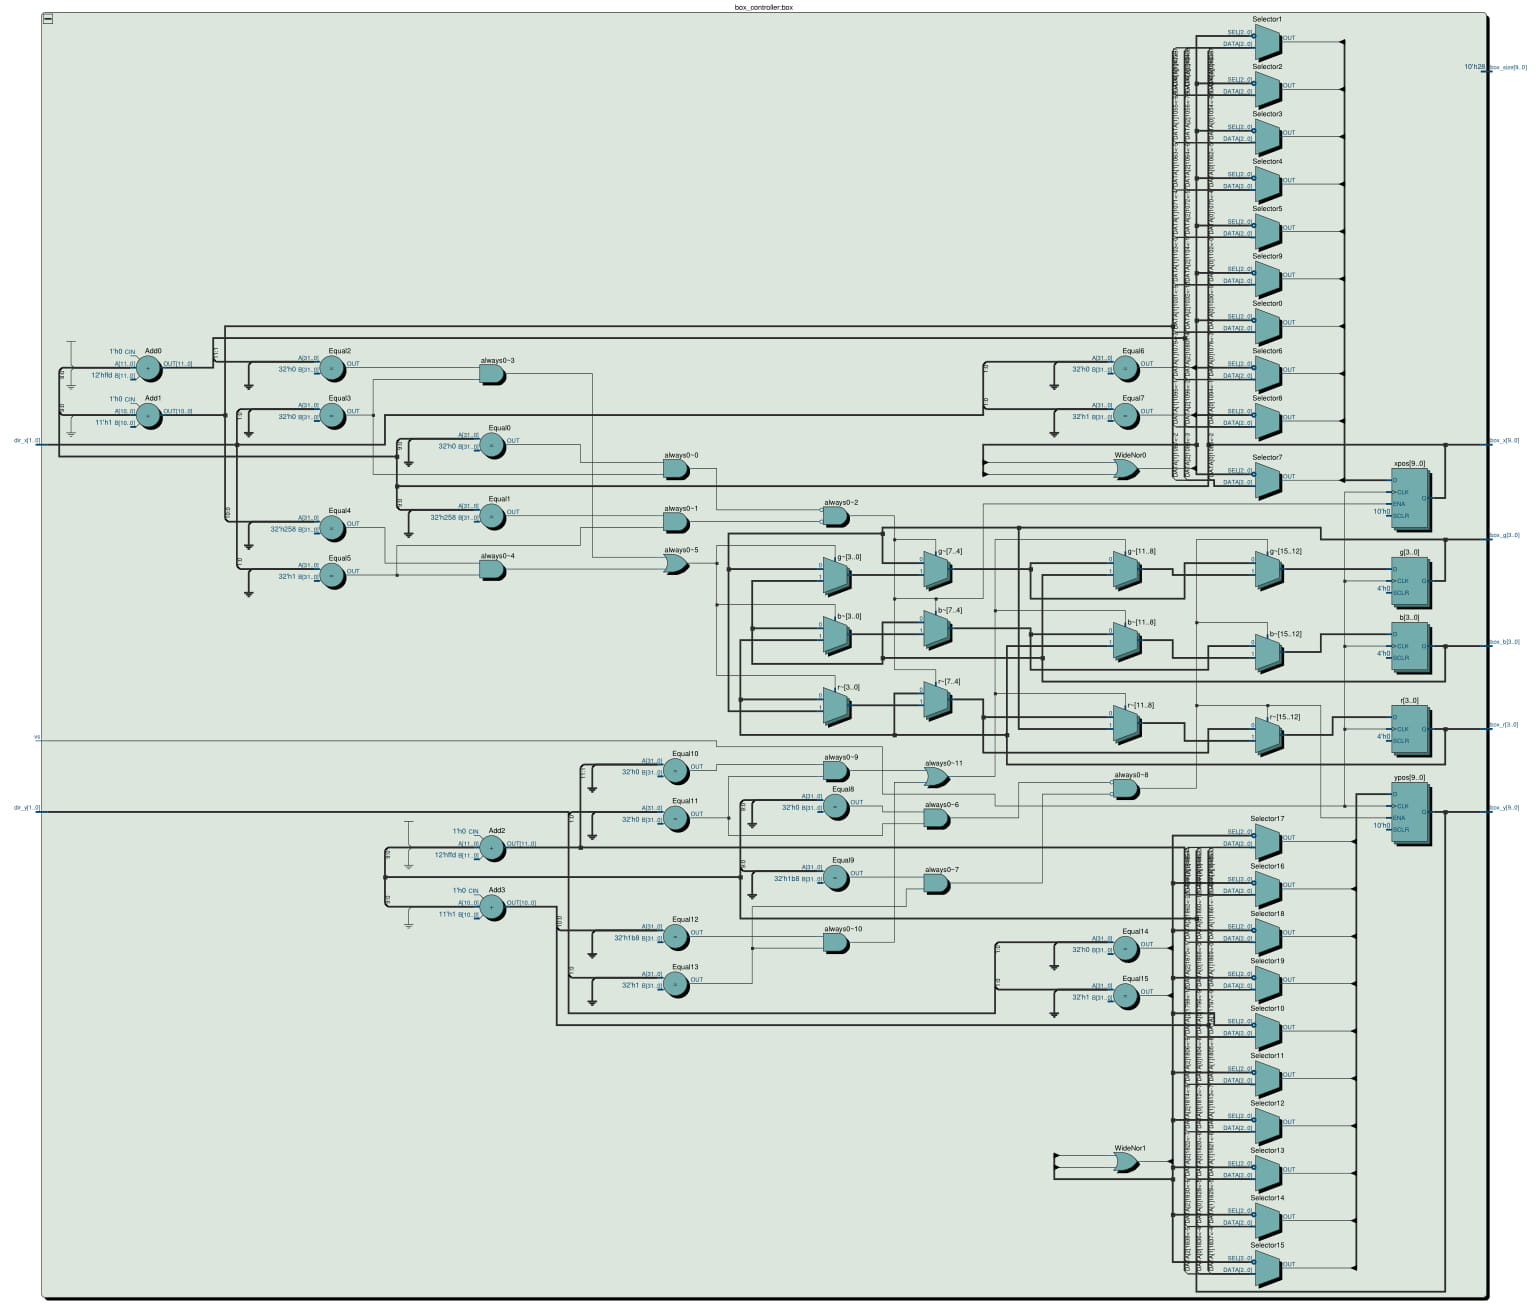
\includegraphics[width=\textwidth]{box_controller.jpg}
  \caption{Box controller module}
  \label{fig:box_controller}
\end{figure}

\begin{figure}[ht]
  \centering
  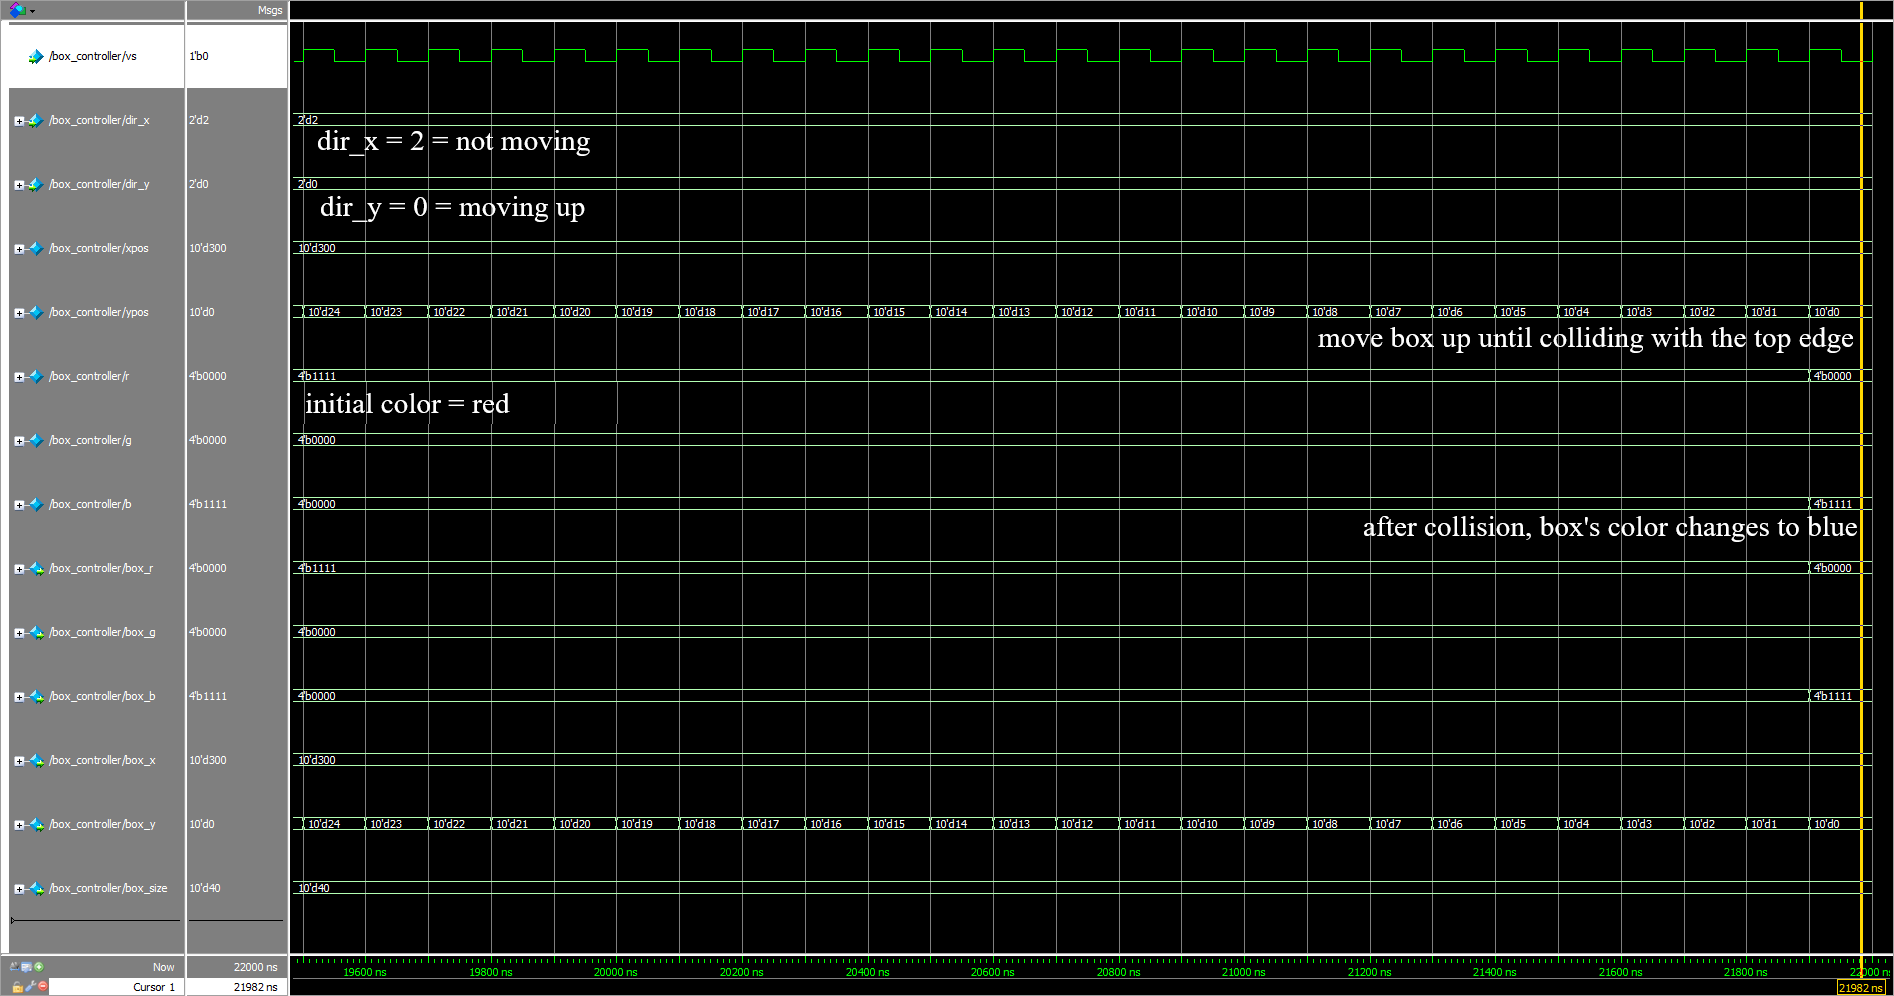
\includegraphics[width=\textwidth]{box_controller_simulation_collision_with_top_edge.png}
  \caption{Box controller module’s simulation testing - Box collides with the top edge of the screen}
  \label{fig:box_controller_simulation_collision_with_top_edge}
\end{figure}

\begin{figure}[ht!]
  \centering
  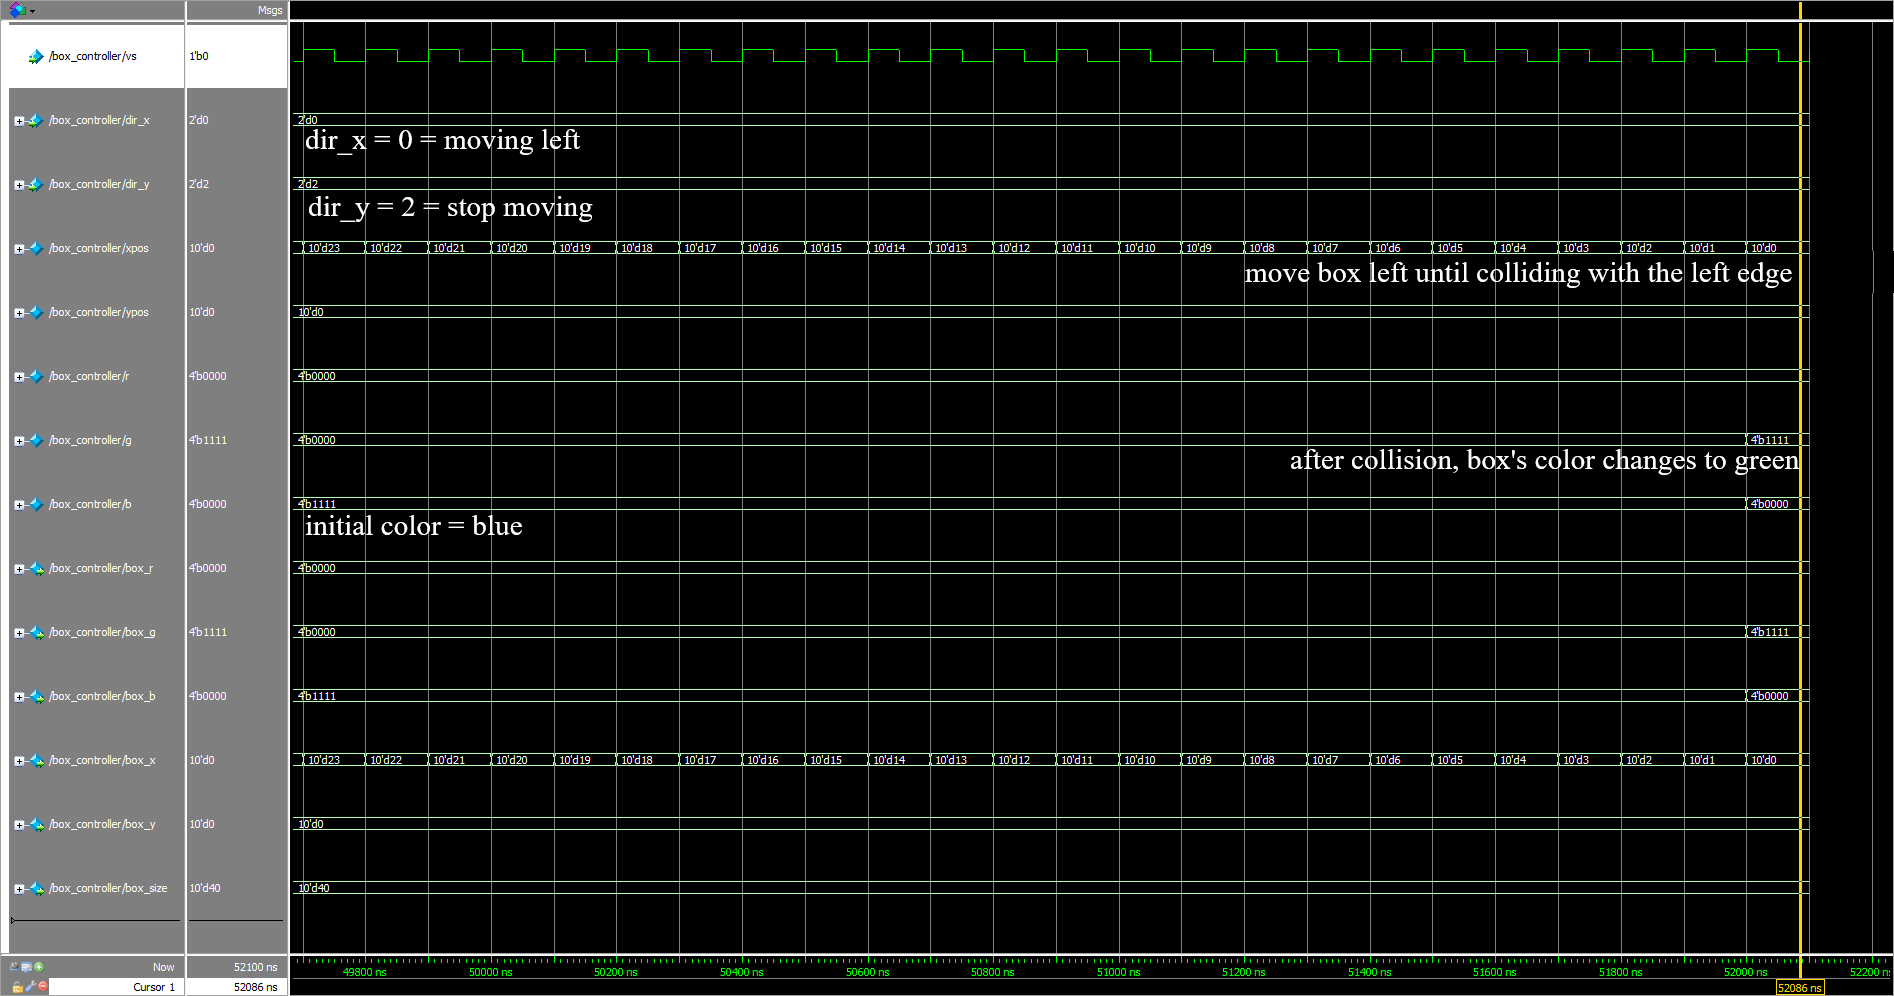
\includegraphics[width=\textwidth]{box_controller_simiulation_collision_with_left_edge.png}
  \caption{Box controller module’s simulation testing - Box collides with the left edge of the screen}
  \label{fig:box_controller_simiulation_collision_with_left_edge}
\end{figure}

\newpage

Inputs: Vertical Sync. $X$ and $Y$ direction in which the box is moving.

Outputs: Three 4-bit buses representing red, green, and blue. Two 10-bit buses representing the and $y$ location of the box.

Description: The Box Controller Module controls the action and animations of the box image. The module takes in 3 inputs representing vertical sync, $X$ direction, and $Y$ direction. $X$ direction and $Y$ specify which direction the box is moving, where 0 represents left or up and 1 represents right or down. The Box Controller checks to ensure that the box will remain in the active pixel range. It then checks to see if a collision with a vertical or horizontal boundary has occurred. If this is true, then the red, green, and blue data lines corresponding to the box are switched, forcing the image to change color. In addition, the box stops moving. For example, if a red box were heading to the right and encounters a collision with the rightmost part of the screen, then the box will change colors to blue, and also stop moving so it does not continue past the edge of the screen. The current state of the box, including its position and color, are outputted to Drawer module.

%%%%%%%%%%%%%%%%%%%%
% XY Counter Module
%%%%%%%%%%%%%%%%%%%%
\subsubsection{XY Counter Module}

\begin{figure}[ht]
  \centering
  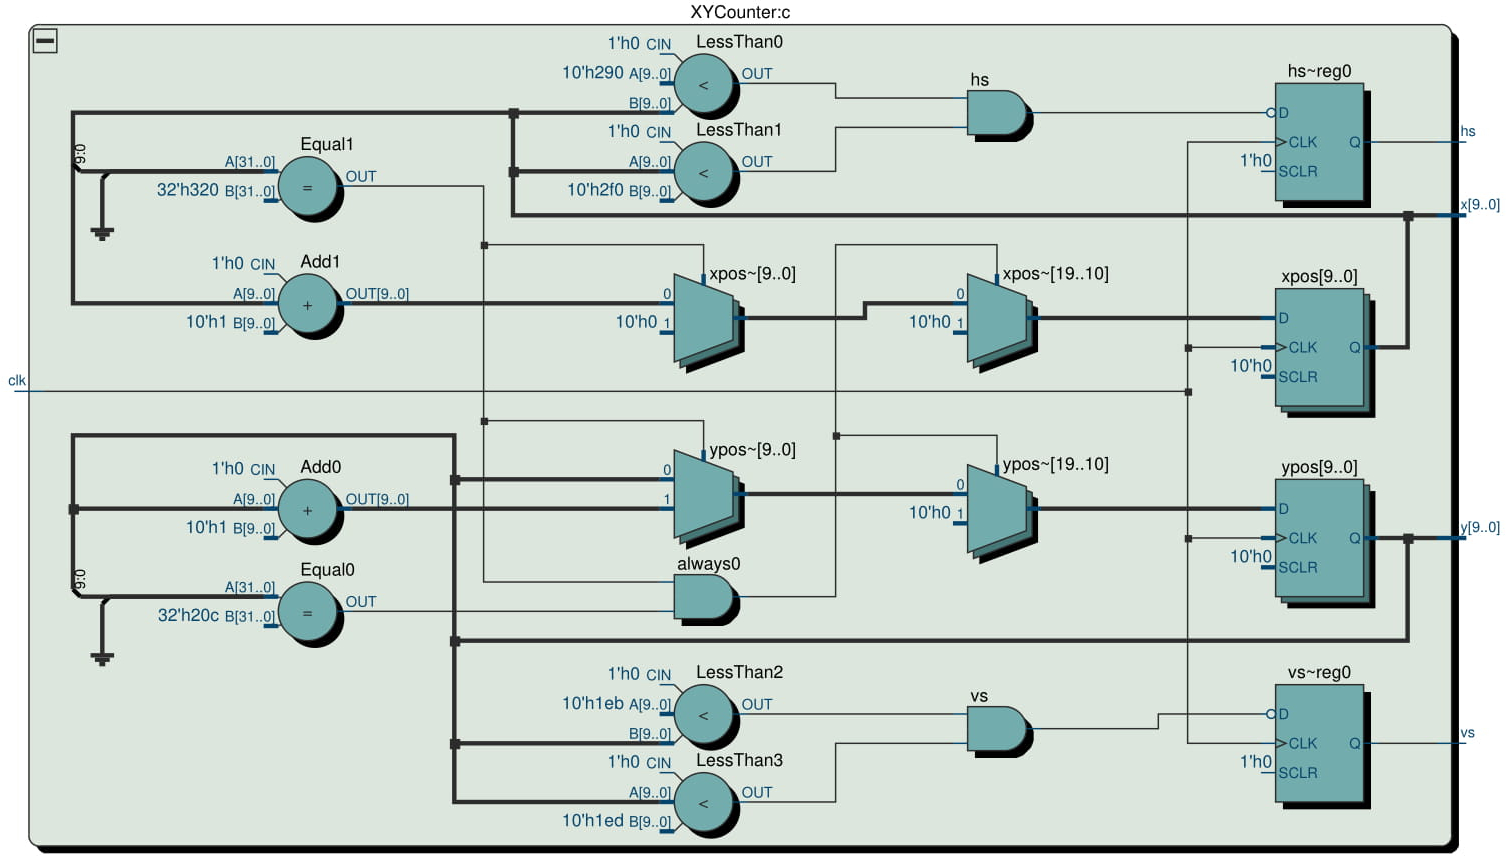
\includegraphics[width=\textwidth]{xycounter.jpg}
  \caption{XY Counter module}
  \label{fig:xycounter}
\end{figure}

\newpage

\begin{figure}[ht]
  \centering
  \includegraphics[width=\textwidth]{xycounter_simulation_horizontal_front_porch.png}
  \caption{XY counter module’s simulation testing - Horizontal front porch}
  \label{fig:xycounter_simulation_horizontal_front_porch}
\end{figure}

\begin{figure}[ht]
  \centering
  \includegraphics[width=\textwidth]{xycounter_simulation_horizontal_sync_pulse.png}
  \caption{XY counter module’s simulation testing - Horizontal sync pulse}
  \label{fig:xycounter_simulation_horizontal_sync_pulse}
\end{figure}

\begin{figure}[ht!]
  \centering
  \includegraphics[width=\textwidth]{xycounter_simulation_horizontal_back_porch.png}
  \caption{XY counter module’s simulation testing - Horizontal back porch and counter completes one line}
  \label{fig:xycounter_simulation_horizontal_back_porch}
\end{figure}

\newpage

\begin{figure}[ht]
  \centering
  \includegraphics[width=\textwidth]{xycounter_simulation_vertical_front_porch.png}
  \caption{XY counter module’s simulation testing - Vertical front porch}
  \label{fig:xycounter_simulation_vertical_front_porch}
\end{figure}

\begin{figure}[ht]
  \centering
  \includegraphics[width=\textwidth]{xycounter_simulation_vertical_sync_pulse.png}
  \caption{XY counter module’s simulation testing - Vertical sync pulse}
  \label{fig:xycounter_simulation_vertical_sync_pulse}
\end{figure}

\begin{figure}[ht!]
  \centering
  \includegraphics[width=\textwidth]{xycounter_simulation_vertical_back_porch.png}
  \caption{XY Counter module’s simulation testing - Vertical back porch and counter completes one screen}
  \label{fig:xycounter_simulation_vertical_back_porch}
\end{figure}

Inputs: Clock

Outputs: Vertical Sync and Horizontal Sync. Two 10-bit buses representing the current $x$ and $y$ pixel location.

Description: The XY Counter module plays a critical role in outputting data as a VGA image. Its purpose is to keep track of horizontal (x) and vertical (y) values to track the pixel position. The module takes only one input, which is the clock, and outputs values for HSync, VSync, and $x$ and $y$ positions. By looking at Figure~\ref{fig:xycounter}, HSync and VSync values are calculated and then outputted directly to the VGA. The $x$ representing the pixel position is continuously incremented until it reaches 800, which signifies a new frame, during which $y$ is initialized and incremented by one. At the same time, $x$ is reset to 0 and incremented again to 800. This process repeats until $y$ reaches 524, which signifies the end of the screen. At this moment, both $x$ and $y$ are reset to 0. The XY Counter module outputs the $x$ and $y$ location to the Drawer module.

%%%%%%%%%%%%%%%%%%%%
% Drawer Module
%%%%%%%%%%%%%%%%%%%%
\subsubsection{Drawer Module}

\begin{figure}[ht]
  \centering
  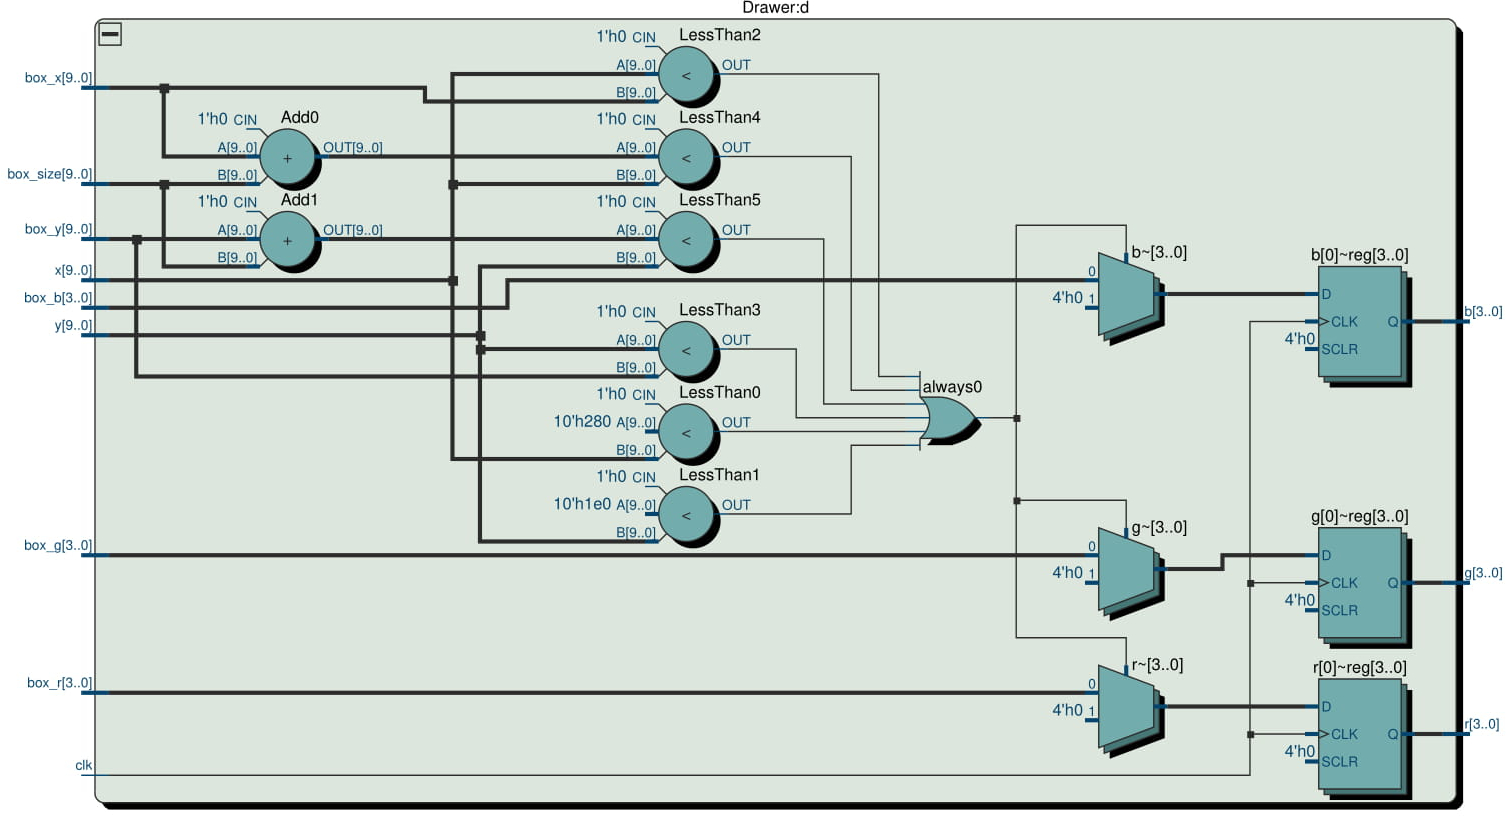
\includegraphics[width=\textwidth]{drawer.jpg}
  \caption{Drawer module}
  \label{fig:drawer}
\end{figure}

\begin{figure}[ht]
  \centering
  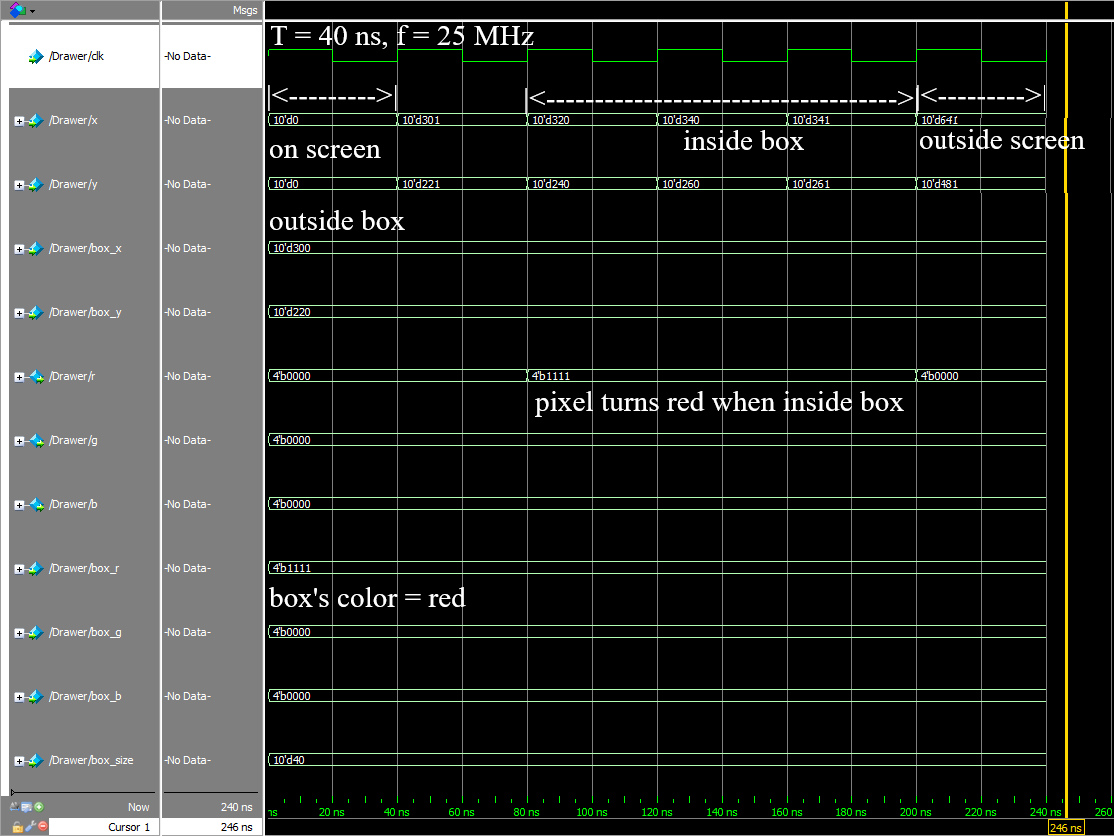
\includegraphics[width=\textwidth]{drawer_simulation.png}
  \caption{Drawer module’s simulation testing - Different pixel colors at different coordinates}
  \label{fig:drawer_simulation}
\end{figure}

Inputs: Three 4-bit buses representing red, green, and blue. $X$ and $Y$ counter as well as $x$ and $y$ locations of the box.

Outputs: Three 4-bit buses representing red, green, and blue.

Description: The Drawer module shown above is the last step in displaying the output as a VGA image. This module reads in data corresponding to the $x$ and $y$ locations that are outputted from the XY Counter module as well as $x$ and $y$ values indicating the size of the box to be displayed. If the $x$ and $y$ locations outputted from the counter module are not within the active pixel range specified by the VGA timing specifications, then a black box is drawn, effectively showing nothing. However, if the location of $x$ and $y$ are within the active pixel range, then the outputs: red, green, and blue, are assigned values so that a colorful box image appear on the monitor. This box will appear at the specified box $x$ and $y$ values, and will have a size specified by the inputs. If the current pixel is outside the location of the box, black is displayed, otherwise either red, green, or blue are displayed to form the box.

\newpage

%%%%%%%%%%%%%%%%%%%%%%%%%%%%%%%%%%%%%%%%%%%%%%%%%%%%%%%%%%%%%%%%%%%%%%%%%%%%%%%%
% Putting It All Together
%%%%%%%%%%%%%%%%%%%%%%%%%%%%%%%%%%%%%%%%%%%%%%%%%%%%%%%%%%%%%%%%%%%%%%%%%%%%%%%%
\section{Putting It All Together}

\begin{figure}[ht]
  \centering
  \includegraphics[width=\textwidth]{ps2_top_level_simulation_dataw_box_starts_moving_up.png}
  \caption{PS/2 Top Level module’s simulation testing - Box starts moving up after receiving a W keypress}
  \label{fig:ps2_top_level_simulation_dataw_box_starts_moving_up}
\end{figure}

\newpage

\begin{figure}[ht]
  \centering
  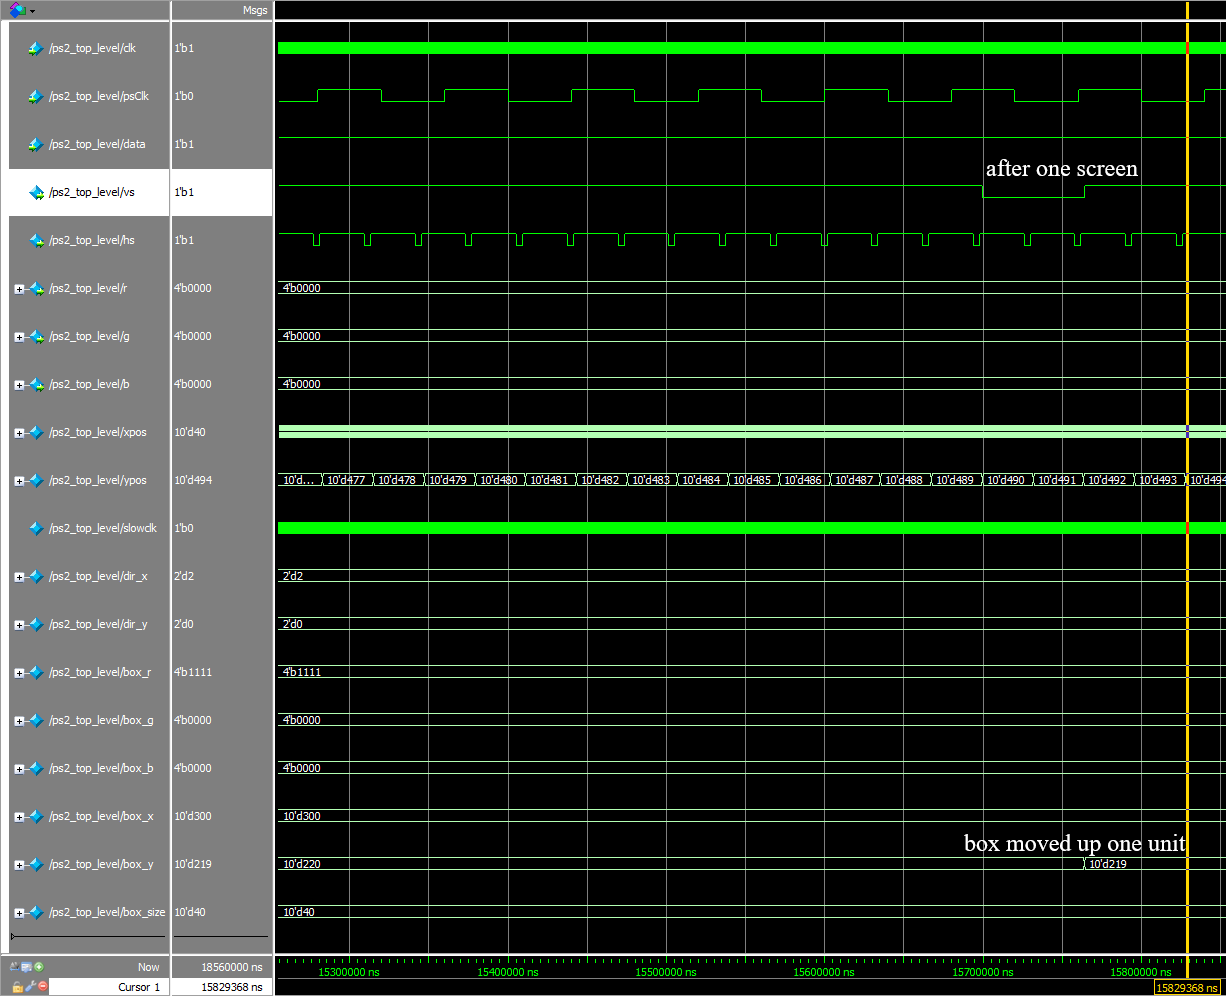
\includegraphics[width=\textwidth]{ps2_top_level_simulation_box_move_up_one_unit.png}
  \caption{PS/2 Top Level module’s simulation testing - Box has moved up 1 pixel. For the remaining 219 pixels the box has left before colliding with the screen, it moves in the same way}
  \label{fig:ps2_top_level_simulation_box_move_up_one_unit}
\end{figure}

\newpage

\begin{figure}[ht]
  \centering
  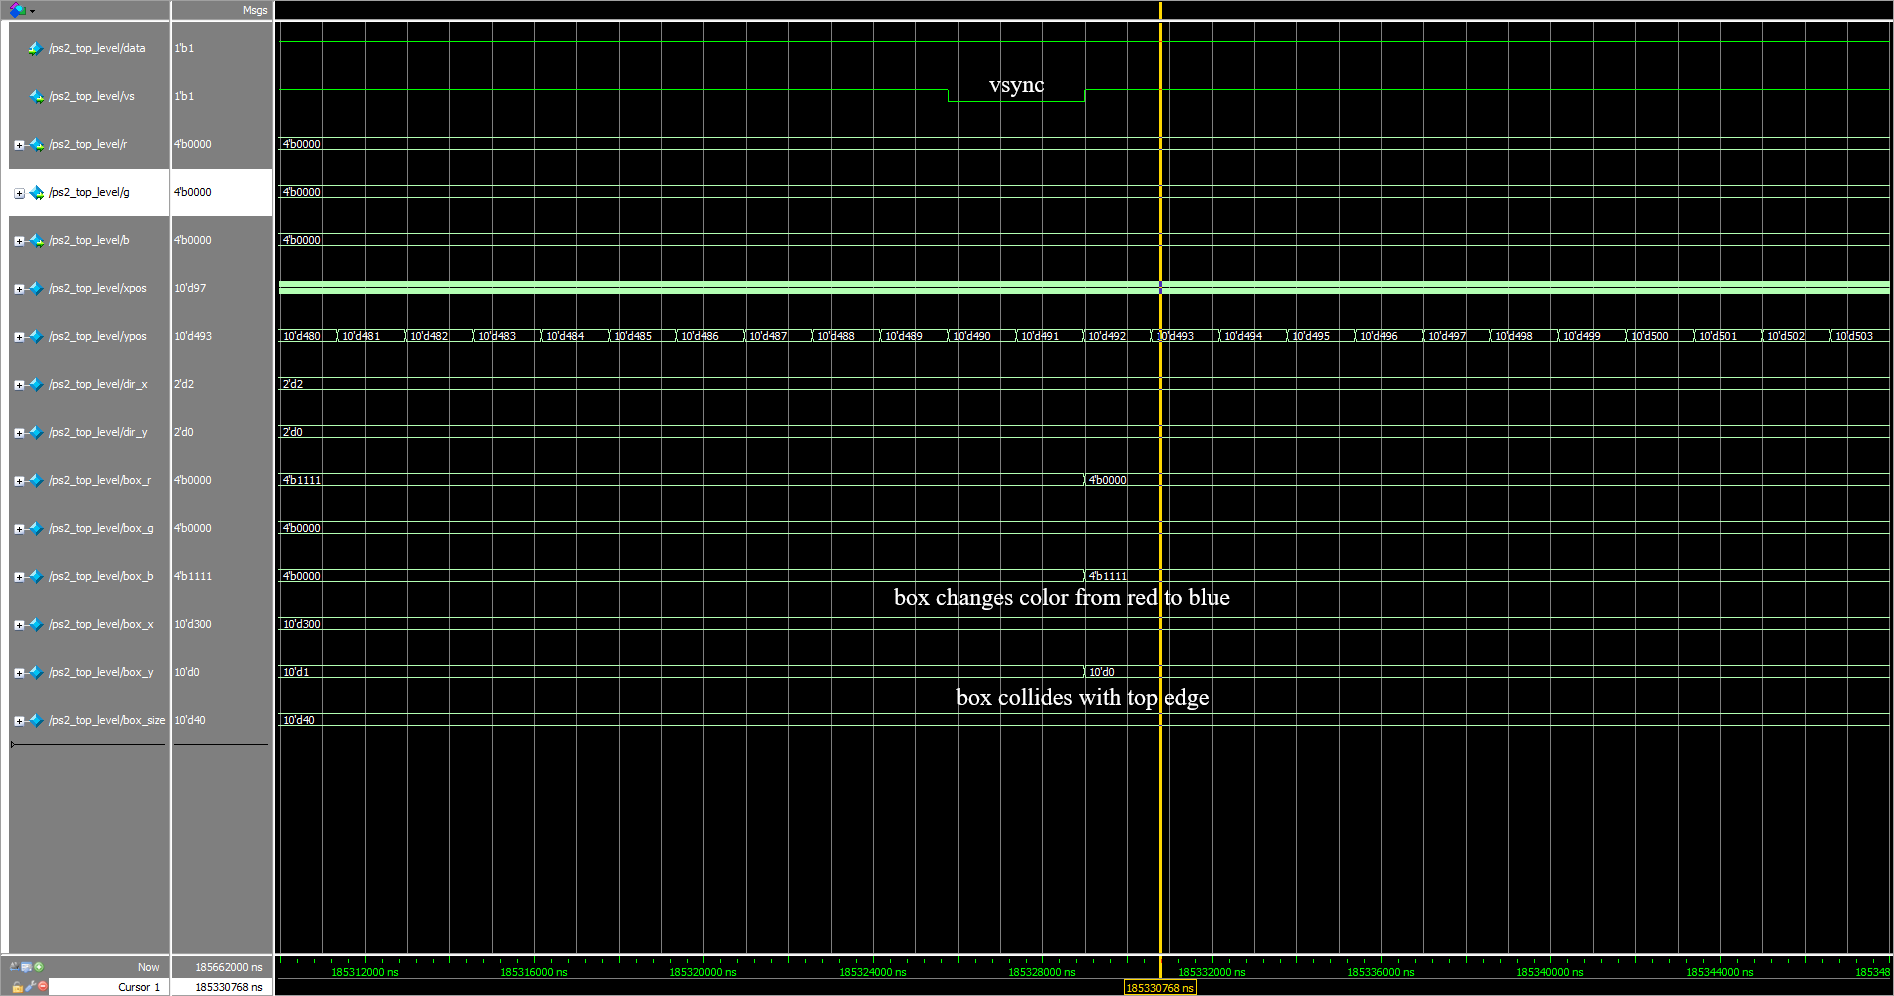
\includegraphics[width=\textwidth]{ps2_top_level_simulation_box_changes_color_collision.png}
  \caption{PS/2 Top Level module’s simulation testing - Box changes color when colliding with the screen}
  \label{fig:ps2_top_level_simulation_box_changes_color_collision}
\end{figure}

Since our group decided to implement all three modes of input, constructing this project was essentially like creating three designs with several commonalities. In each design, the XY Counter, Half Clock, Box Controller, and Drawer modules were all used in transferring data from the FPGA to a VGA output. The one difference between each design was implementation of the decoder module. Each unique form of input needed a separate decoder module that was able to read and transmit data correctly from the controller to the other modules within the FPGA. A top level HDL file was made for all three modes of input and tested thoroughly using ModelSim.

%%%%%%%%%%%%%%%%%%%%%%%%%%%%%%%%%%%%%%%%%%%%%%%%%%%%%%%%%%%%%%%%%%%%%%%%%%%%%%%%
% Above and Beyond
%%%%%%%%%%%%%%%%%%%%%%%%%%%%%%%%%%%%%%%%%%%%%%%%%%%%%%%%%%%%%%%%%%%%%%%%%%%%%%%%
\section{Above and Beyond}

After looking at the rubric, our group decided to take it one step further by accomplishing all of the tasks listed on the rubric. We successfully implemented VGA output using all three forms of input: PS/2, RC5 IR, and NES. In addition, we attempted to animate the behavior of the outputted image, rather than having a static and plain figure. By adding the box controller module, we included logic that would force the image to change color and direction upon one condition. If the box hit the edge of the active pixel range, whether in the horizontal or vertical direction, then it would change color. In addition to changing color, the box stops moving, creating a collision.

%%%%%%%%%%%%%%%%%%%%%%%%%%%%%%%%%%%%%%%%%%%%%%%%%%%%%%%%%%%%%%%%%%%%%%%%%%%%%%%%
% Appendix
%%%%%%%%%%%%%%%%%%%%%%%%%%%%%%%%%%%%%%%%%%%%%%%%%%%%%%%%%%%%%%%%%%%%%%%%%%%%%%%%
\section{Appendix}

\subsection{SystemVerilog Source Code}

\subsubsection{Top Level}

\inputminted[breaklines, fontfamily=tt, fontsize=\small, frame=lines, framesep=1.5em, linenos, numbersep=1.5em, style=vs]{systemverilog}{../src/top_level.sv}

\subsubsection{PS/2 Top Level}

\inputminted[breaklines, fontfamily=tt, fontsize=\small, frame=lines, framesep=1.5em, linenos, numbersep=1.5em, style=vs]{systemverilog}{../src/ps2_top_level.sv}

\subsubsection{PS/2 Controller}

\inputminted[breaklines, fontfamily=tt, fontsize=\small, frame=lines, framesep=1.5em, linenos, numbersep=1.5em, style=vs]{systemverilog}{../src/ps2.sv}

\subsubsection{RC5 IR Top Level}

\inputminted[breaklines, fontfamily=tt, fontsize=\small, frame=lines, framesep=1.5em, linenos, numbersep=1.5em, style=vs]{systemverilog}{../src/ir_top_level.sv}

\subsubsection{RC5 IR Controller}

\inputminted[breaklines, fontfamily=tt, fontsize=\small, frame=lines, framesep=1.5em, linenos, numbersep=1.5em, style=vs]{systemverilog}{../src/ir.sv}

\subsubsection{NES Top Level}

\inputminted[breaklines, fontfamily=tt, fontsize=\small, frame=lines, framesep=1.5em, linenos, numbersep=1.5em, style=vs]{systemverilog}{../src/nes_top_level.sv}

\subsubsection{NES Controller}

\inputminted[breaklines, fontfamily=tt, fontsize=\small, frame=lines, framesep=1.5em, linenos, numbersep=1.5em, style=vs]{systemverilog}{../src/nes.sv}

\subsubsection{Box Controller}

\inputminted[breaklines, fontfamily=tt, fontsize=\small, frame=lines, framesep=1.5em, linenos, numbersep=1.5em, style=vs]{systemverilog}{../src/box_controller.sv}

\subsubsection{Half Clock}

\inputminted[breaklines, fontfamily=tt, fontsize=\small, frame=lines, framesep=1.5em, linenos, numbersep=1.5em, style=vs]{systemverilog}{../src/half_clock.sv}

\subsubsection{XY Counter}

\inputminted[breaklines, fontfamily=tt, fontsize=\small, frame=lines, framesep=1.5em, linenos, numbersep=1.5em, style=vs]{systemverilog}{../src/XYCounter.sv}

\subsubsection{Drawer}

\inputminted[breaklines, fontfamily=tt, fontsize=\small, frame=lines, framesep=1.5em, linenos, numbersep=1.5em, style=vs]{systemverilog}{../src/Drawer.sv}

\end{document}
